% !TeX program = xelatex
% !TeX encoding = UTF-8

\documentclass[10pt]{article}

\usepackage{fontspec}
\setmainfont[
  Path = fonts/,
  UprightFont = CharisSIL-Regular.ttf,
  BoldFont = CharisSIL-Bold.ttf,
  ItalicFont = CharisSIL-Italic.ttf,
  BoldItalicFont = CharisSIL-BoldItalic.ttf
]{Charis SIL}

\usepackage{geometry}
\geometry{
  paperwidth=192mm,
  paperheight=262mm,
  left=13.75mm,
  right=13.75mm,
  top=17.4mm,
  bottom=18.0mm,
  headheight=10pt,
  headsep=7pt,
  footskip=9.5mm
}

\usepackage{amsmath, amssymb}
\usepackage{xcolor}
\usepackage{graphicx}
\usepackage{url}

\definecolor{jfdscyan}{HTML}{0a80ad}
\usepackage[colorlinks=true, linkcolor=jfdscyan, citecolor=jfdscyan, urlcolor=jfdscyan]{hyperref}

\renewcommand{\figurename}{Fig.}
\renewcommand{\tablename}{Table}

% Pure LaTeX booktabs-style rules without external packages (expandable before \noalign)
\def\jfdsTopRule{\noalign{\hrule height 0.7pt\vskip 2pt}}
\def\jfdsMidRule{\noalign{\vskip 1.5pt\hrule height 0.4pt\vskip 2pt}}
\def\jfdsBotRule{\noalign{\vskip 1.5pt\hrule height 0.7pt}}

% Pure LaTeX caption, Harvard Author-Year citation, and footnote styling matching JFDS
\makeatletter
\def\@tabcaptype{table}
\long\def\@makecaption#1#2{%
  \vskip\abovecaptionskip
  \ifx\@captype\@tabcaptype
    {\raggedright\fontsize{7.2pt}{9.6pt}\selectfont\textbf{#1}\\#2\par}%
  \else
    {\fontsize{7.2pt}{9.6pt}\selectfont\textbf{#1.} #2\par}%
  \fi
  \vskip\belowcaptionskip}
\def\figcaption{\def\@captype{figure}\caption}

% Footnote separator rule matching Elsevier JFDS short top rule
\renewcommand\footnoterule{\kern-3pt \hrule width 0.28\linewidth height 0.4pt \kern 2.6pt}

% Pure LaTeX Harvard Author-Year \citep / \citet + unnumbered JFDS hanging-indent bibliography
\def\@citeloop#1,#2\@nil{%
  \edef\@ckey{\zap@space#1 \@empty}%
  \@ifundefined{bibauth@\@ckey}{\textbf{?}}{\hyperlink{cite.\@ckey}{\csname bibauth@\@ckey\endcsname, \csname bibyear@\@ckey\endcsname}}%
  \if\relax\detokenize{#2}\relax\else; \@citeloop#2\@nil\fi
}
\def\@citetloop#1,#2\@nil{%
  \edef\@ckey{\zap@space#1 \@empty}%
  \@ifundefined{bibauth@\@ckey}{\textbf{?}}{\hyperlink{cite.\@ckey}{\csname bibauth@\@ckey\endcsname\ (\csname bibyear@\@ckey\endcsname)}}%
  \if\relax\detokenize{#2}\relax\else, \@citetloop#2\@nil\fi
}
\DeclareRobustCommand{\citep}[1]{(\@citeloop#1,\@nil)}
\DeclareRobustCommand{\citet}[1]{\@citetloop#1,\@nil}

\renewenvironment{thebibliography}[1]{%
  \raggedbottom
  \section*{\refname}%
  \list{}{%
    \setlength{\leftmargin}{12pt}%
    \setlength{\itemindent}{-12pt}%
    \setlength{\itemsep}{1.0pt}%
    \setlength{\parsep}{0pt}%
    \setlength{\parskip}{0pt}%
    \setlength{\topsep}{0pt}%
    \setlength{\partopsep}{0pt}%
    \usecounter{enumiv}%
    \let\p@enumiv\@empty
    \renewcommand\theenumiv{\relax}%
  }%
  \def\bibitem[##1(##2)]##3{%
    \item\leavevmode\hypertarget{cite.##3}{}%
    \immediate\write\@auxout{\string\global\string\@namedef{bibauth@##3}{\unexpanded{##1}}}%
    \immediate\write\@auxout{\string\global\string\@namedef{bibyear@##3}{\unexpanded{##2}}}%
    \ignorespaces}%
  \fontsize{6.6pt}{8.4pt}\selectfont
  \sloppy\clubpenalty4000\widowpenalty4000%
  \sfcode`\.\@m
}{%
  \endlist
}
\def\@biblabel#1{}%
\makeatother

% Standard paragraph indentation and spacing for The Journal of Finance and Data Science
\setlength{\parindent}{12pt}
\setlength{\parskip}{0pt plus 1pt}
\linespread{1.05}
\setlength{\emergencystretch}{1.2em}

% Base font size hierarchy matching The Journal of Finance and Data Science (8.0pt body text)
\renewcommand{\normalsize}{\fontsize{8.0pt}{10.5pt}\selectfont}
\renewcommand{\small}{\fontsize{7.5pt}{9.8pt}\selectfont}
\renewcommand{\footnotesize}{\fontsize{7.2pt}{9.2pt}\selectfont}
\renewcommand{\large}{\fontsize{9.5pt}{12.0pt}\selectfont}
\renewcommand{\Large}{\fontsize{11.5pt}{14.5pt}\selectfont}
\renewcommand{\LARGE}{\fontsize{13.5pt}{17.0pt}\selectfont}

% Optimization of float placement
\renewcommand{\topfraction}{0.88}
\renewcommand{\bottomfraction}{0.80}
\renewcommand{\textfraction}{0.12}
\renewcommand{\floatpagefraction}{0.85}

% Running header and footer matching The Journal of Finance and Data Science
\makeatletter
\def\ps@paperstyle{%
  \def\@oddhead{\fontsize{6.4pt}{8.0pt}\selectfont\textit{H.C. Tran, T.G. Phan}\hfill\textit{The Journal of Finance and Data Science}}%
  \def\@evenhead{\fontsize{6.4pt}{8.0pt}\selectfont\textit{H.C. Tran, T.G. Phan}\hfill\textit{The Journal of Finance and Data Science}}%
  \def\@oddfoot{\hfil\fontsize{6.4pt}{8.0pt}\selectfont\thepage\hfil}%
  \def\@evenfoot{\hfil\fontsize{6.4pt}{8.0pt}\selectfont\thepage\hfil}%
}
\def\ps@firstpage{%
  \def\@oddhead{}%
  \def\@evenhead{}%
  \def\@oddfoot{\hfil\fontsize{6.4pt}{8.0pt}\selectfont\thepage\hfil}%
  \def\@evenfoot{\hfil\fontsize{6.4pt}{8.0pt}\selectfont\thepage\hfil}%
}
% Section and Subsection Formatting matching The Journal of Finance and Data Science
\renewcommand{\@seccntformat}[1]{\csname the#1\endcsname.\ }
\renewcommand\section{\@startsection {section}{1}{\z@}%
                                   {-2.8ex \@plus -0.8ex \@minus -.3ex}%
                                   {1.0ex \@plus .2ex}%
                                   {\normalfont\bfseries\fontsize{8.5pt}{11.0pt}\selectfont}}
\renewcommand\subsection{\@startsection{subsection}{2}{\z@}%
                                     {-2.0ex\@plus -0.5ex \@minus -.2ex}%
                                     {0.7ex \@plus .2ex}%
                                     {\normalfont\itshape\fontsize{8.0pt}{10.5pt}\selectfont}}
\renewcommand\subsubsection{\@startsection{subsubsection}{3}{\z@}%
                                     {-1.5ex\@plus -0.4ex \@minus -.2ex}%
                                     {0.4ex \@plus .1ex}%
                                     {\normalfont\itshape\fontsize{7.8pt}{10.0pt}\selectfont}}
\makeatother
\pagestyle{paperstyle}

\begin{document}
\thispagestyle{firstpage}

% ==============================================================================
% JOURNAL HEADER BANNER (THE JOURNAL OF FINANCE AND DATA SCIENCE / ELSEVIER / KEAI)
% ==============================================================================
\noindent
\includegraphics[width=\textwidth]{pictures/jfds_header_banner_complete.pdf}\par
\vspace{8pt}

% Research Article Badge (Charis SIL Regular 9.5pt)
\noindent{\fontsize{9.5pt}{12pt}\selectfont Research Article}\par
\vspace{4pt}

% Article Title (Charis SIL Regular 13.5pt - Generous leading and spacing before authors)
\noindent{\fontsize{13.5pt}{17.5pt}\selectfont Velocity-Adaptive versus Quantum-Behaved Particle Swarm Optimization for Neural Network Hyperparameter Tuning: An Empirical Comparative Study\par}
\vspace{9pt}

% Author Block with Given Middle Surname order & cyan superscripts matching sample JFDS
\noindent{\fontsize{10.5pt}{13pt}\selectfont Hung Cuong Tran\textsuperscript{\textcolor{jfdscyan}{a,*}}, Truong Giang Phan\textsuperscript{\textcolor{jfdscyan}{a}}}\par
\vspace{5pt}
\noindent{\fontsize{6.4pt}{8.5pt}\selectfont\textit{\textsuperscript{a} School of Information and Communication Technology, Hanoi University of Industry, Hanoi, Vietnam}\par}
\begingroup
\makeatletter
\long\def\@makefntext#1{\noindent\hspace*{6pt}#1}
\makeatother
\footnotetext{%
\textsuperscript{*} Corresponding author.\\
\hspace*{6pt}\textit{E-mail addresses:} \href{mailto:tranhungcuong@haui.edu.vn}{tranhungcuong@haui.edu.vn} (H.C. Tran), \href{mailto:2023606481@st.haui.edu.vn}{2023606481@st.haui.edu.vn} (T.G. Phan).%
}
\endgroup

\vspace{16pt}

% ==============================================================================
% ARTICLE INFO & ABSTRACT (ELSEVIER / KEAI JFDS 2-COLUMN BOX - NO VERTICAL RULE)
% ==============================================================================
\noindent\rule{\textwidth}{0.4pt}\par\vspace{3pt}
\noindent\begin{minipage}[t]{0.265\textwidth}
{\fontsize{7.0pt}{9.0pt}\selectfont A R T I C L E \quad I N F O}\par\vspace{2pt}
\rule{\linewidth}{0.4pt}\par\vspace{5pt}
{\fontsize{6.4pt}{8.6pt}\selectfont\textit{Keywords:}}\par\vspace{2pt}
{\fontsize{6.4pt}{8.6pt}\selectfont
Particle Swarm Optimization\\
Quantum-behaved PSO\\
Hyperparameter tuning\\
Multilayer Perceptron\\
Loss landscape exploration\\
Tabular classification\par}
\end{minipage}%
\hspace{0.035\textwidth}%
\begin{minipage}[t]{0.70\textwidth}
{\fontsize{7.0pt}{9.0pt}\selectfont A B S T R A C T}\par\vspace{2pt}
\rule{\linewidth}{0.4pt}\par\vspace{5pt}
{\fontsize{7.2pt}{9.6pt}\selectfont
Hyperparameter selection critically governs the generalization capability of artificial neural networks, yet empirical validation landscapes remain rugged, non-convex, and corrupted by stochastic initialization noise. While standard Particle Swarm Optimization (PSO) provides competitive baseline search capability, particles frequently suffer from premature stagnation and trajectory instability. To investigate these dynamics, this study presents a unified cross-paradigm benchmark evaluating fifteen PSO algorithms spanning velocity-adaptive Newtonian dynamics---including constriction-based tuning inspired by Optimized Particle Swarm Optimization (OPSO)---and quantum-behaved potential-well mechanisms that eliminate velocity vectors. Evaluated across Multilayer Perceptron (MLP) architecture and regularization tuning on Bank Marketing ($N=11{,}162$) and a stratified Forest Covertype subsample ($N=30{,}000$), velocity-adaptive Linear Decay inertia (LD-PSO, $85.80\%$) and Fractional-Order momentum (FO-PSO, $85.62\%$, achieving a $41.59\%$ hidden-unit reduction) consistently rank highest across tasks. Within the quantum paradigm, elite-centroid Q-MBPSO ($85.62\%$ on Bank) and annealed Q-LDPSO ($85.42\%$ on Covertype) sustain productive delta-well tunneling, whereas canonical QPSO with unweighted all-particle centroids degrades on Bank Marketing ($83.48\%$). These findings indicate that structured velocity damping and elite-guided quantum contraction improve holdout generalization under modest $240$-evaluation budgets.\par}
\end{minipage}\par\vspace{4pt}
\noindent\rule{\textwidth}{0.4pt}\par\vspace{10pt}







\section{Introduction}

Hyperparameter optimization (HPO) critically governs the representational capacity and generalization performance of artificial neural networks~\citep{feurer2019hyperparameter}. Tuning continuous and integer parameters—such as hidden layer widths, learning rates, and regularization penalties—remains fundamentally challenging. Empirical validation landscapes are non-convex, rugged, and corrupted by stochastic noise from data partitioning and random weight initialization. Because these objective surfaces lack analytical gradients across architecture choices, practitioners routinely compare random and sequential Bayesian surrogates~\citep{bergstra2012random,snoek2012practical} against gradient-free, population-based metaheuristics, among which Particle Swarm Optimization (PSO)~\citep{kennedy1995particle,poli2007particle} represents a prominent paradigm.

Standard PSO coordinates a swarm of candidate solutions through Newtonian kinematic equations, balancing individual historical success against collective swarm memory~\citep{trelea2003particle,vandenbergh2006study}. Although standard PSO converges rapidly during early iterations, particles frequently suffer from velocity explosion or collapse into suboptimal local attractors. To mitigate premature stagnation, algorithmic research has branched into velocity-adaptive Newtonian dynamics---spanning dynamic inertia schedules, constriction factors, and fractional-order memory~\citep{bansal2011inertia,nickabadi2011novel,ratnaweera2004self,chatterjee2006nonlinear}---and velocity-free Quantum-behaved PSO (QPSO)~\citep{sun2004global,sun2012quantum}, which models particles as bound states within quantum delta potential wells capable of probabilistic tunneling.

Despite extensive algorithmic developments and recent neural hyperparameter studies~\citep{lorenzo2017particle,junior2019particle,zhang2025large}, a practical comparative gap persists. Much of the optimization literature focuses on idealized synthetic functions or isolated single-variant proposals, leaving the head-to-head trade-offs between Newtonian momentum damping and quantum delta-well contraction largely uncharacterized under identical neural network evaluation budgets. Practitioners still lack controlled empirical evidence comparing classical, fractional, directional, and quantum formulations across distinct tabular dimensionalities.

To address this gap, we establish a unified, budget-constrained benchmarking framework evaluating fifteen PSO algorithms for Multilayer Perceptron (MLP) hyperparameter optimization. Fig.~\ref{fig:flowchart} illustrates the overall architecture. The framework coordinates candidate parameter generation across a bounded three-dimensional manifold, evaluating each configuration through stratified cross-validation~\citep{kohavi1995study}. Particles update their attractor states across successive iterations, branching into either adaptive velocity damping or quantum delta-well sampling. This dual-paradigm formulation permits a direct, controlled contrast between momentum-guided kinematics and probabilistic tunneling on real tabular classification benchmarks.

\begin{figure}[t]
\centering
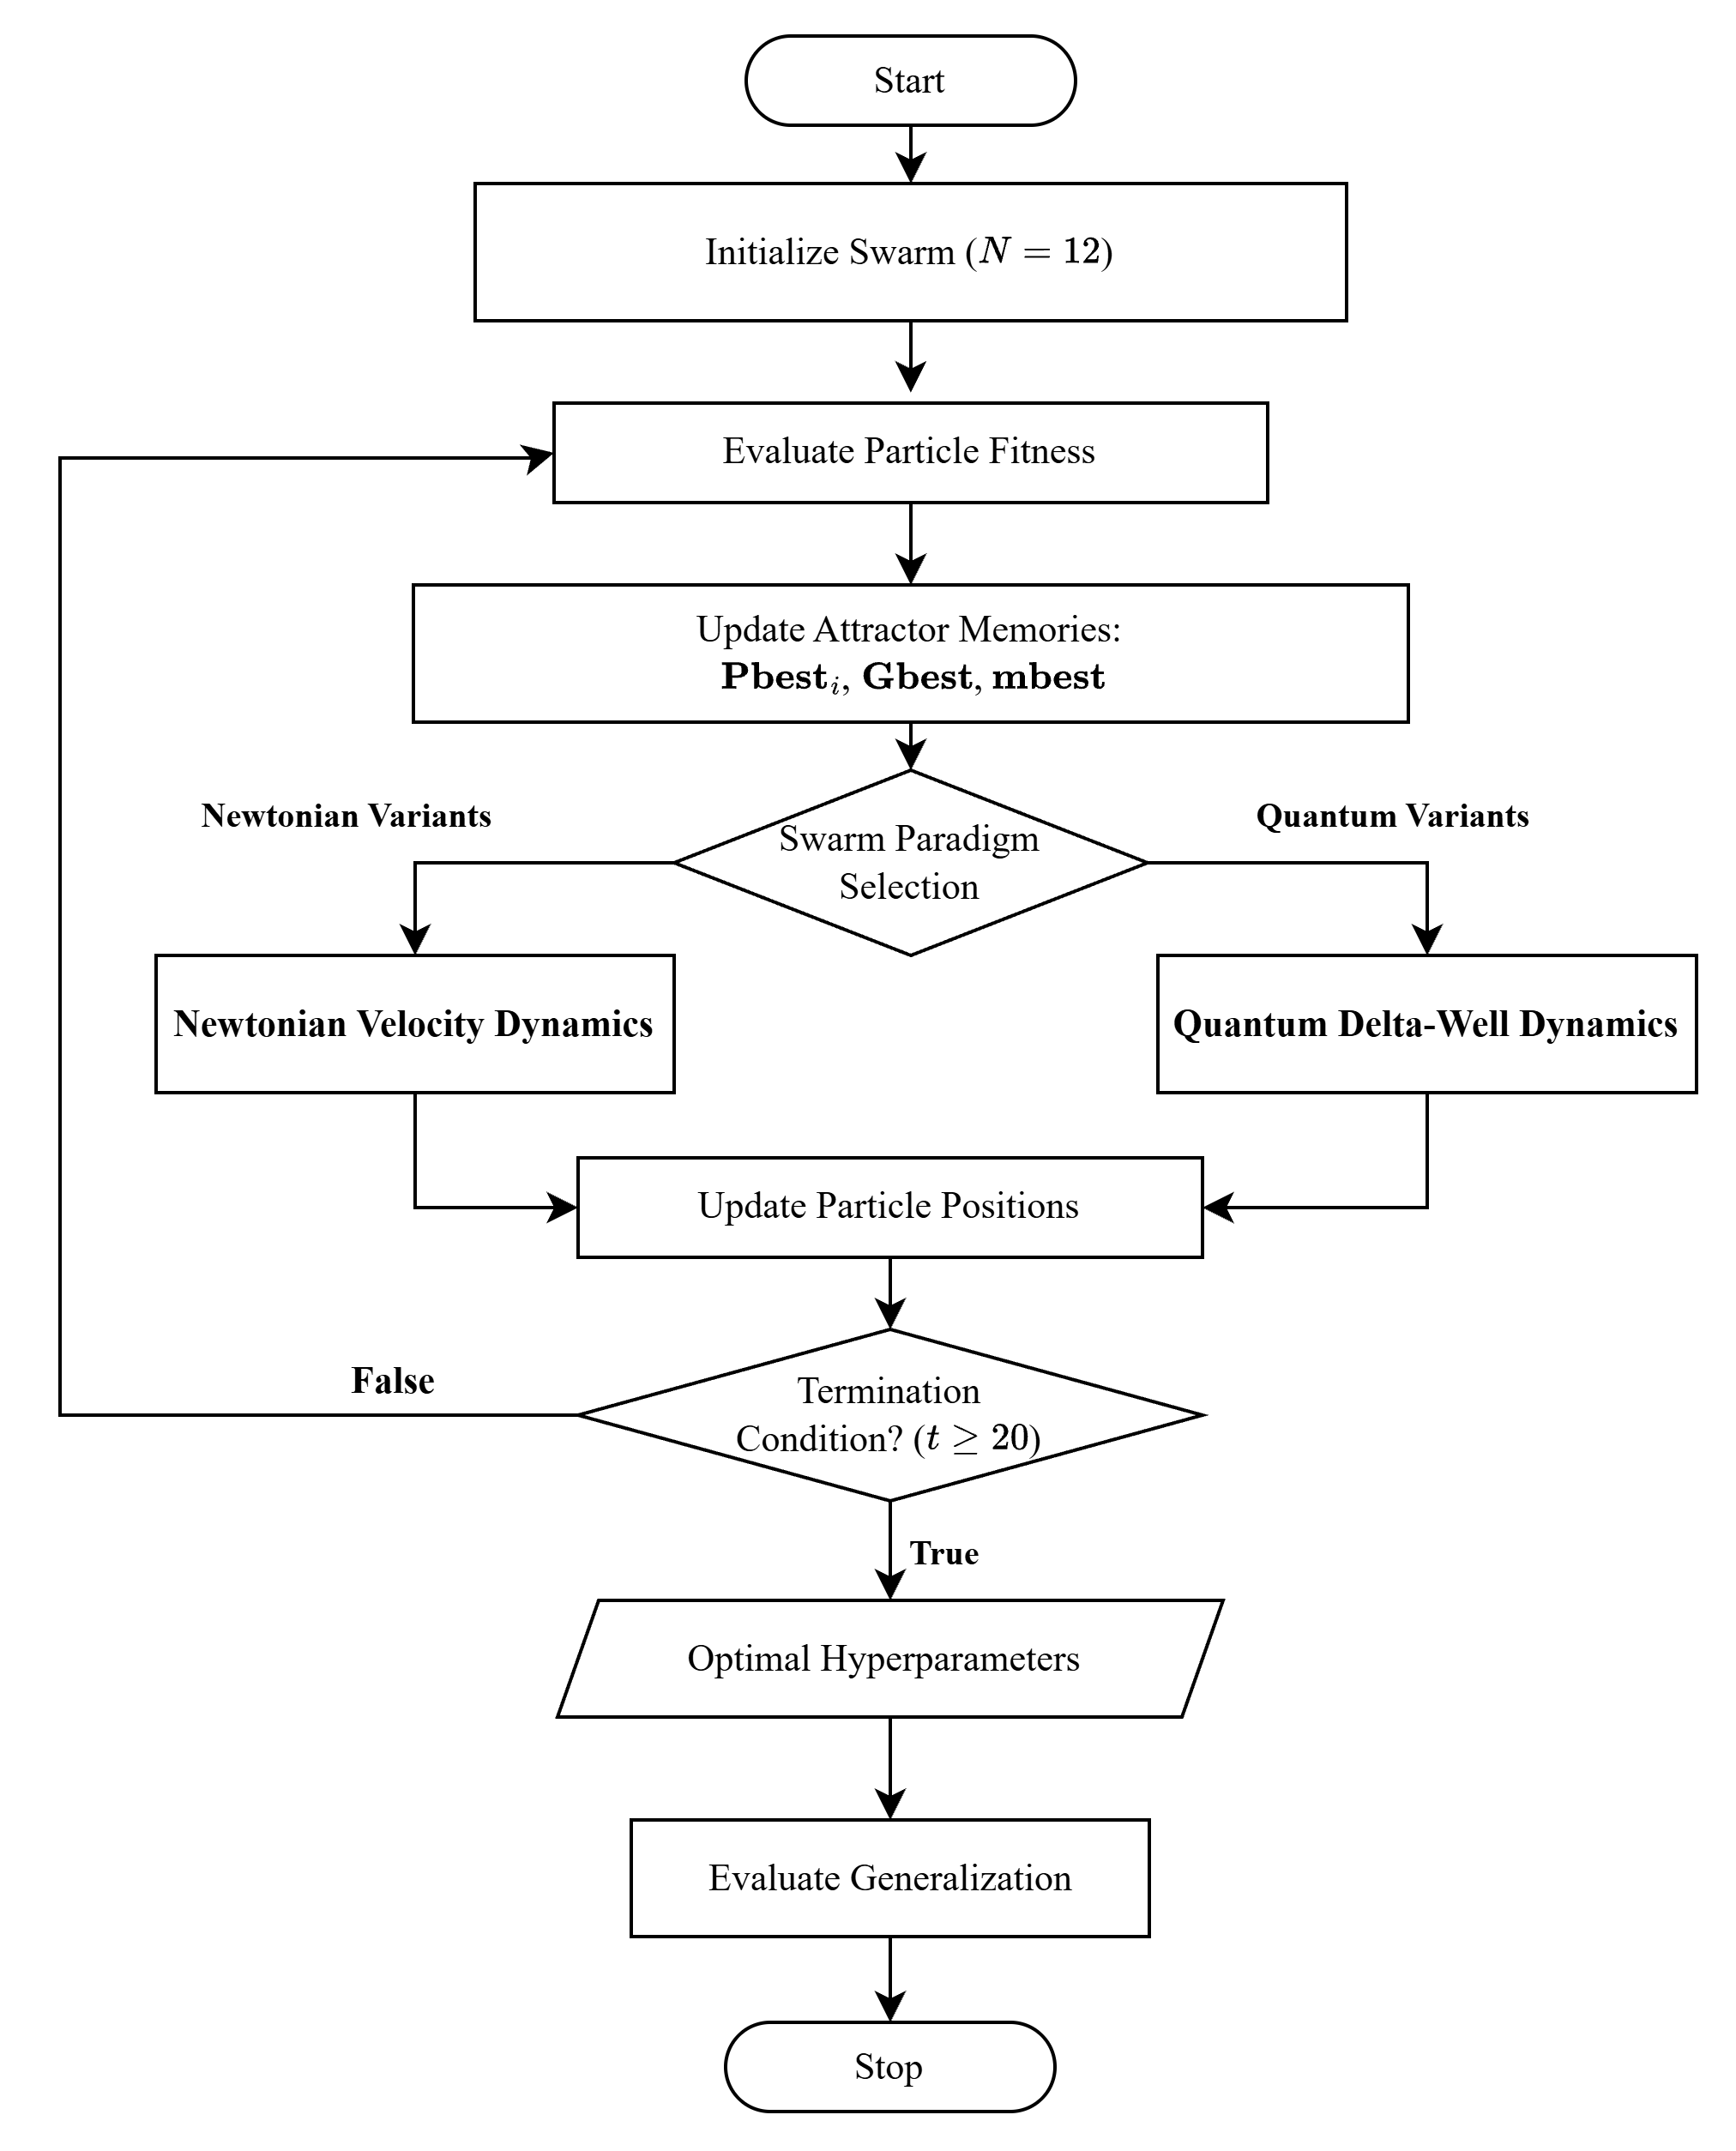
\includegraphics[width=0.58\textwidth]{figures/flowchart.png}
\caption{Flowchart of the unified hyperparameter optimization framework for Multilayer Perceptron (MLP) neural networks, illustrating the cross-validation evaluation loop and the bifurcation between Newtonian velocity-based and Quantum delta-well swarm paradigms.}
\label{fig:flowchart}
\end{figure}

The primary contributions of this paper are fourfold:
\begin{enumerate}
    \item \textbf{Unified Cross-Paradigm Benchmark:} We present a systematic, head-to-head empirical evaluation of fifteen distinct PSO algorithms—spanning eight velocity-adaptive Newtonian variants and seven quantum-behaved formulations—under a standardized stratified 5-fold cross-validation protocol ($N=12$ particles, $T=20$ iterations; $240$ objective evaluations and $1{,}200$ baseline folds per variant, rising to $720$ evaluations for $k_{\mathrm{avg}}=3$ averaging and $312$ for opposition jumping).
    \item \textbf{Mechanistic Trajectory Characterization:} We analyze how adaptive inertia decay, constriction factors, fractional-order velocity memory ($\alpha_{\mathrm{FO}} = 0.6$), and elite vs.\ full-population quantum centroids alter swarm diversity, explaining both CV--test inversions and canonical QPSO dispersion.
    \item \textbf{Dual-Domain Empirical Validation:} We benchmark all variants across two contrasting tabular tasks—the class-balanced \textit{Bank Marketing} benchmark ($N=11{,}162$ records, $16$ raw attributes encoded into $42$ features)~\citep{moro2014data} and a stratified subsample ($N=30{,}000$, representing $5.16\%$ of the $581{,}012$-record corpus) of the 7-class \textit{Forest Covertype} problem ($54$ features)~\citep{blackard1999comparative}—showing that top-performing variants (LD-PSO, FO-PSO, Q-MBPSO, and Q-LDPSO) deliver competitive holdout accuracy ($85.80\%$ and $85.42\%$) alongside compact architectures ($41.59\%$ hidden-unit reduction for FO-PSO on Bank Marketing).
    \item \textbf{Computational Efficiency and Practical Guidelines:} We show that dynamic velocity damping and elite-centroid quantum contraction operate strictly within the baseline $240$-evaluation budget, achieving higher mean rank than brute-force multi-seed trial averaging ($720$ evaluations).
\end{enumerate}

The remainder of this paper is organized as follows. Section~2 formalizes the hyperparameter optimization problem, dataset preprocessing, and fifteen algorithmic variants. Section~3 reports empirical results across both classification benchmarks. Section~4 discusses convergence mechanisms, loss surface geometry, adjacent AutoML trade-offs, and threats to validity. Finally, Section~5 concludes the paper and highlights avenues for future work.

\section{Proposed Method}

The optimization of Multilayer Perceptron (MLP) hyperparameters is formulated over a bounded continuous search space $\Omega \subset \mathbb{R}^3$. Each particle in the swarm represents a candidate solution vector $X_i = [x_{i,1}, x_{i,2}, x_{i,3}]^T$ mapped directly to the architectural and regularization hyperparameters of a ReLU-activated MLP implemented in \textit{scikit-learn}~\citep{pedregosa2011scikit}:
\begin{align}
n_{\mathrm{neurons}} &= \operatorname{clip}(\operatorname{round}(x_{i,1}), \, 16, \, 256), \quad x_{i,1} \in [16, 256] \label{eq:decode_n} \\
\eta &= 10^{x_{i,2}}, \quad x_{i,2} \in [-4.0, -1.0] \label{eq:decode_lr} \\
\alpha &= 10^{x_{i,3}}, \quad x_{i,3} \in [-5.0, -1.0] \label{eq:decode_alpha}
\end{align}
where $n_{\mathrm{neurons}}$ defines the number of hidden units in each layer of a two-hidden-layer architecture $(n_{\mathrm{neurons}}, n_{\mathrm{neurons}})$, $\eta$ specifies the initial learning rate of the Adam optimizer~\citep{kingma2014adam}, and $\alpha$ represents the L2 regularization penalty coefficient. Logarithmic scaling is applied to $\eta$ and $\alpha$ to allow uniform sampling across multiple orders of magnitude.

To evaluate the generalization quality of candidate configuration $\theta(X_i) = \langle n_{\mathrm{neurons}}, \eta, \alpha \rangle$ without overfitting the training set, the fitness objective function $f(X_i)$ is defined as the mean classification accuracy obtained through Stratified 5-Fold Cross-Validation~\citep{kohavi1995study}:
\begin{equation}
f(X_i) = \frac{1}{K} \sum_{k=1}^K \mathrm{Accuracy}_k(\mathrm{MLP}(\theta(X_i))), \quad K=5 \label{eq:fitness}
\end{equation}
During each training fit, \texttt{MLPClassifier} reserves an internal stratified $10\%$ validation split (\texttt{validation\_fraction=0.1}) and applies early stopping monitored on validation accuracy, halting if no improvement exceeds \texttt{tol}=$10^{-4}$ within \texttt{n\_iter\_no\_change}=15 consecutive epochs (capped at \texttt{max\_iter}=500 during cross-validation and Bank Marketing holdout evaluation, and \texttt{max\_iter}=1000 with patience 20 during final Covertype holdout evaluation).

\subsection{Benchmark Datasets and Experimental Protocol}

All fifteen PSO variants are evaluated on two public tabular classification tasks preprocessed under an identical deterministic train--test partition (\texttt{RANDOM\_SEED=42}, $80\% / 20\%$ stratified split) with continuous features standardized via \texttt{StandardScaler} fit strictly on the training fold~\citep{pedregosa2011scikit,hastie2009elements}:
\begin{itemize}
    \item \textbf{Bank Marketing (Binary):} Sourced from the curated balanced CSV release ($N = 11{,}162$ instances: $5{,}873$ negative [$52.6\%$] and $5{,}289$ positive [$47.4\%$])~\citep{moro2014data}. Encoding the $16$ raw attributes via one-hot dummy indicators (\texttt{drop\_first=True}) produces a $42$-dimensional feature space split into $8{,}929$ training and $2{,}233$ holdout test samples.
    \item \textbf{Forest Covertype (7-Class):} Derived from the $581{,}012$-sample cartographic corpus across $54$ continuous and binary soil/wilderness indicators~\citep{blackard1999comparative}. To keep cross-validation tractable across $15$ algorithms ($\approx 20{,}760$ CV fits per dataset), experiments use a fixed stratified subsample of $N = 30{,}000$ instances ($5.16\%$ of the full corpus), partitioned into $24{,}000$ training and $6{,}000$ holdout test samples.
\end{itemize}

\subsection{Standard Particle Swarm Optimization}

Standard Particle Swarm Optimization (Standard PSO), introduced by \citet{kennedy1995particle}, coordinates a swarm of $N=12$ particles navigating the three-dimensional search space $\Omega$. In each iteration $t$, the velocity vector $V_i(t) \in \mathbb{R}^3$ and position vector $X_i(t) \in \mathbb{R}^3$ of particle $i$ are updated by integrating inertial momentum with cognitive and social cognitive attractors:
\begin{equation}
V_i(t+1) = w \cdot V_i(t) + c_1 \cdot r_1 \cdot (Pbest_i(t) - X_i(t)) + c_2 \cdot r_2 \cdot (Gbest(t) - X_i(t)) \label{eq:pso_velocity}
\end{equation}
\begin{equation}
X_i(t+1) = X_i(t) + V_i(t+1) \label{eq:pso_position}
\end{equation}
where $w = 0.7$ denotes the constant inertia weight; $c_1 = 1.5$ and $c_2 = 1.5$ represent the cognitive and social acceleration coefficients, respectively; and $r_1, r_2 \sim \mathcal{U}(0,1)^3$ are uniformly distributed random vectors. The vector $Pbest_i(t)$ stores the historical best position discovered by particle $i$, while $Gbest(t)$ designates the global best position found across the entire swarm.

To prevent particle trajectories from diverging uncontrollably beyond search limits, velocity clamping is enforced component-wise with a dynamic threshold $V_{\max} = \gamma \cdot (X_{\max} - X_{\min})$, where $\gamma = 0.2$:
\begin{equation}
v_{i,d}(t+1) = \max(-V_{\max,d}, \, \min(v_{i,d}(t+1), \, V_{\max,d})), \quad d \in \{1, 2, 3\} \label{eq:v_clamp}
\end{equation}
Similarly, position boundaries are strictly constrained to remain within feasible hyperparameter ranges:
\begin{equation}
x_{i,d}(t+1) = \max(X_{\min,d}, \, \min(x_{i,d}(t+1), \, X_{\max,d})), \quad d \in \{1, 2, 3\} \label{eq:pos_clamp}
\end{equation}
Following position updates and fitness evaluations, the cognitive memory $Pbest_i$ and social memory $Gbest$ are updated greedily:
\begin{align}
Pbest_i(t+1) &= \begin{cases} X_i(t+1), & \text{if } f(X_i(t+1)) > f(Pbest_i(t)) \\ Pbest_i(t), & \text{otherwise} \end{cases} \label{eq:pbest_update} \\
Gbest(t+1) &= \arg\max_{Pbest_i} f(Pbest_i(t+1)) \label{eq:gbest_update}
\end{align}

Fig.~\ref{fig:standard_pso_flowchart} illustrates the complete operational workflow of Standard PSO applied to the neural network hyperparameter tuning framework.

\begin{figure}[htbp]
\centering
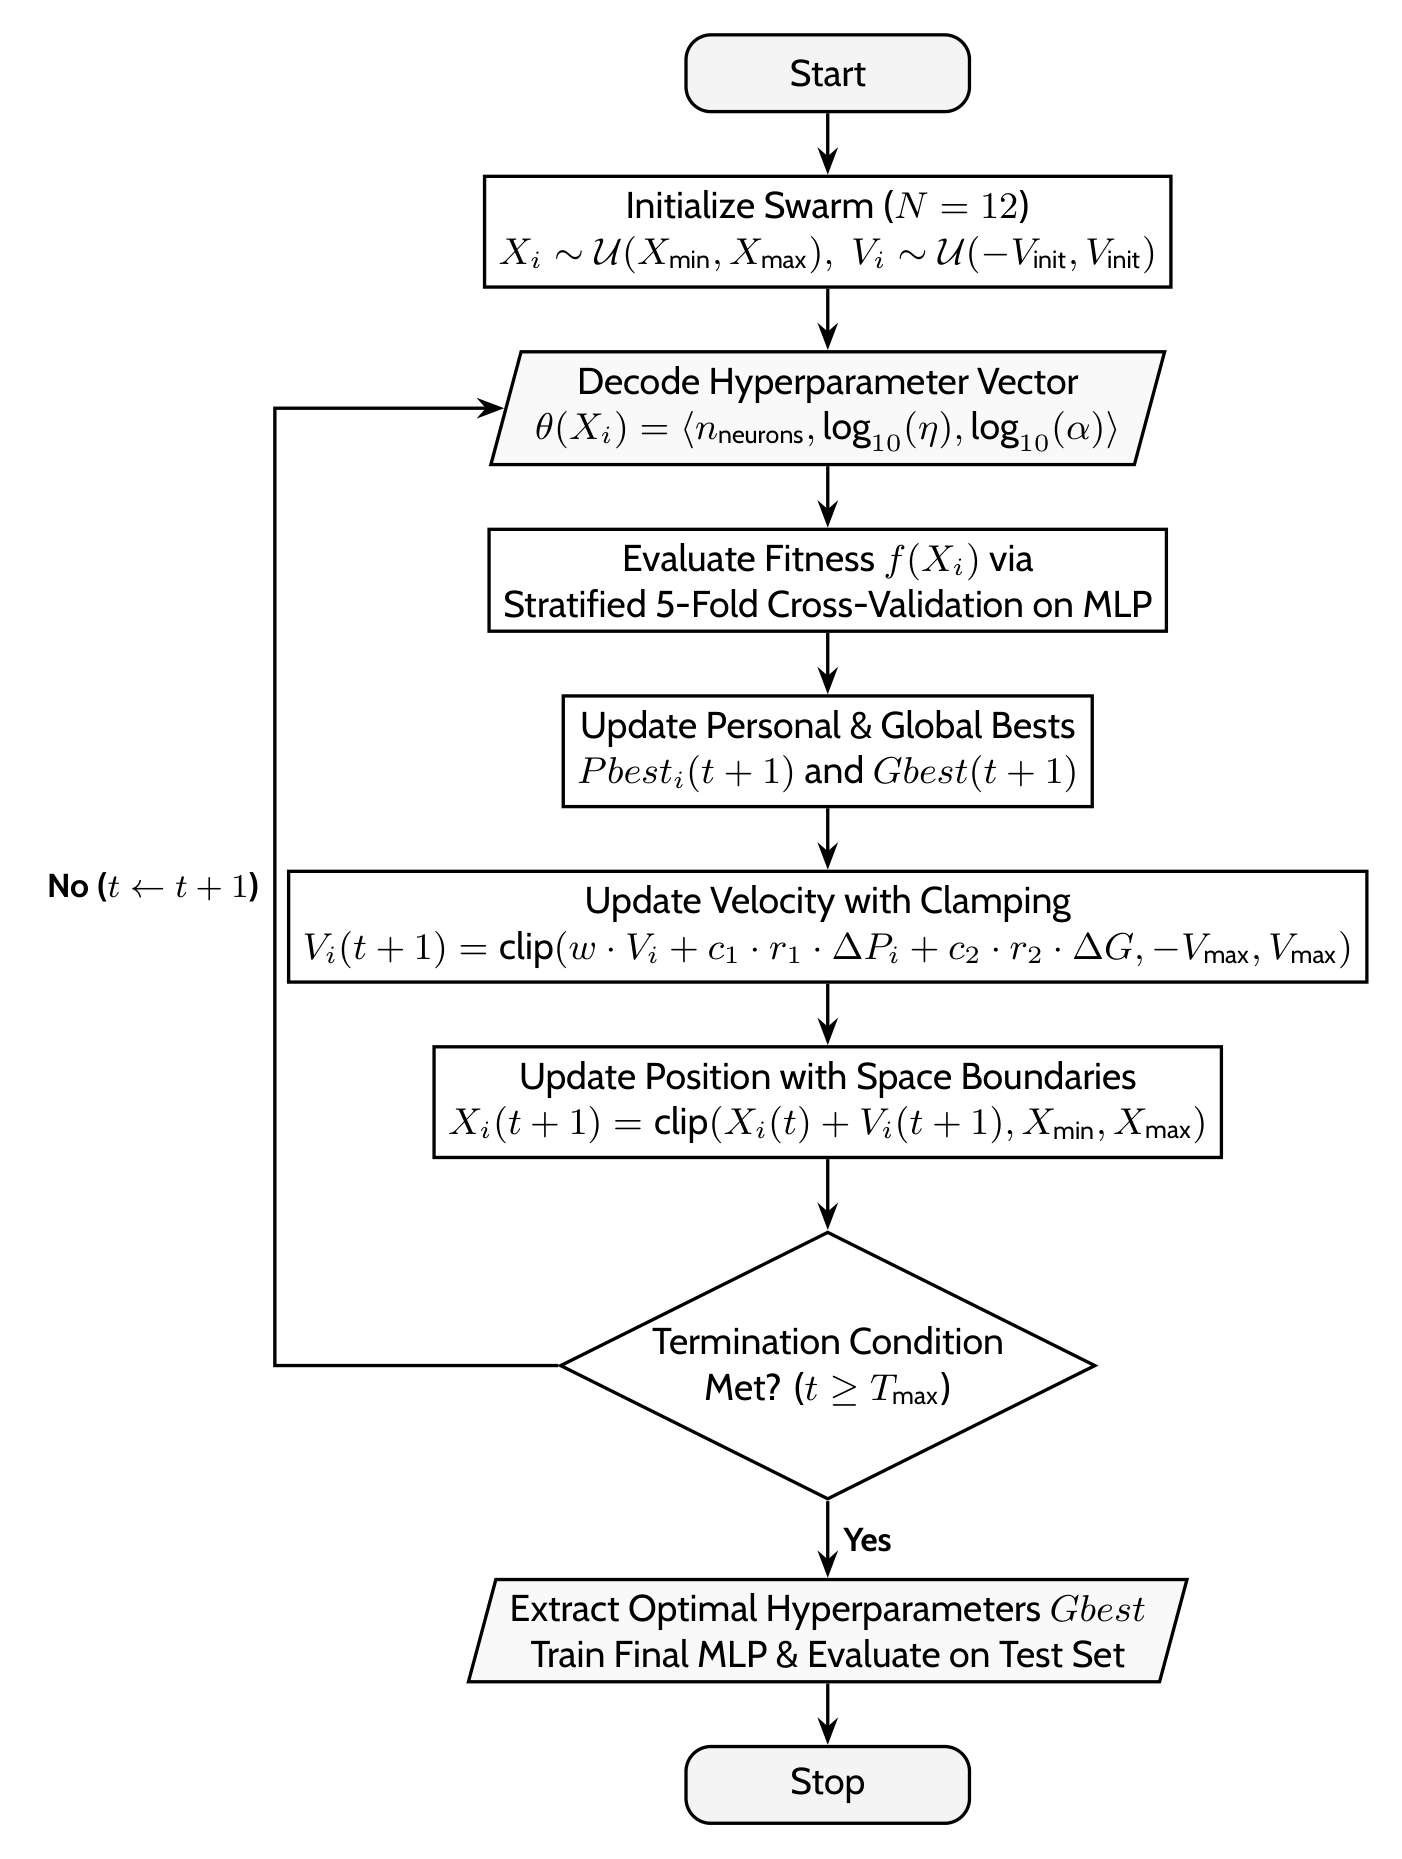
\includegraphics[width=0.41\textwidth]{figures/standard_pso_flowchart.png}
\caption{Flowchart of the baseline Standard Particle Swarm Optimization (Standard PSO) for neural network hyperparameter tuning, detailing the iterative sequence from swarm initialization, hyperparameter decoding, stratified 5-fold cross-validation, velocity clamping, and boundary enforcement to final holdout model evaluation.}
\label{fig:standard_pso_flowchart}
\end{figure}





\subsection{Proposed PSO Enhancements}

To address the susceptibility of Standard PSO to premature stagnation and erratic exploration in complex, non-convex hyperparameter landscapes, this study investigates enhanced swarm mechanisms. We structure these advancements across two fundamental paradigms: (i) \textit{Velocity-Adaptive Swarm Optimization}, which refines Newtonian inertia, trajectory directionality, and social attraction; and (ii) \textit{Quantum-Behaved Swarm Optimization}, which eliminates velocity vectors entirely in favor of wave-packet probability collapse.


\subsubsection*{Linear Decay Inertia Weight (LD-PSO) \citep{shi1998modified}}

In standard swarm dynamics, a static inertia weight ($w = 0.7$) maintains an invariant ratio between inertial momentum and localized attraction across iterations. In rugged neural network hyperparameter landscapes, this static setting creates an acute empirical dilemma: a large fixed inertia induces persistent oscillations that overshoot narrow optimal basins during late generations, whereas a small fixed inertia induces premature swarm collapse into suboptimal architectural topologies during early epochs.

To resolve this conflict, Linear Decay Particle Swarm Optimization (LD-PSO) incorporates a dynamically decelerating inertia schedule:
\begin{equation}
w(t) = w_{\mathrm{start}} - \left(\frac{w_{\mathrm{start}} - w_{\mathrm{end}}}{T}\right) \cdot t \label{eq:linear_decay}
\end{equation}
where $w_{\mathrm{start}} = 0.9$ facilitates wide-ranging exploratory leaps across disparate network configurations during early epochs ($t \ll T$), $w_{\mathrm{end}} = 0.4$ parameterizes the target floor (reaching $w(19) = 0.425$ at the final index $t = 19$ under denominator $T=20$), $t \in \{0, 1, \dots, T-1\}$ denotes the discrete iteration index, and $T = 20$ represents the maximum iteration budget. The velocity vector of particle $i$ is updated as:
\begin{equation}
V_i(t+1) = w(t) \cdot V_i(t) + c_1 \cdot r_1 \odot (Pbest_i(t) - X_i(t)) + c_2 \cdot r_2 \odot (Gbest(t) - X_i(t)) \label{eq:ldpso_velocity}
\end{equation}
while maintaining fixed cognitive ($c_1 = 1.5$) and social ($c_2 = 1.5$) acceleration coefficients with stochastic vectors $r_1, r_2 \sim \mathcal{U}(0,1)^3$ and $\odot$ denoting element-wise (Hadamard) multiplication. Component-wise velocity clamping $V_{\max} = \gamma \cdot (X_{\max} - X_{\min})$ with $\gamma = 0.2$ and boundary projections are enforced identically to Equations~\eqref{eq:v_clamp} and \eqref{eq:pos_clamp}, ensuring that kinetic momentum decays smoothly without boundary divergence.


\subsubsection*{Noise-Resilient Fitness Averaging (FA-PSO)}

Stochastic gradient backpropagation combined with pseudo-random weight initializations introduces severe evaluation noise into neural network hyperparameter landscapes. In single-shot cross-validation schemes, candidate evaluations suffer from high sample variance: a mediocre hyperparameter combination may attain an artificially elevated validation score due to a fortuitously initialized weight seed, whereas a globally superior architecture may be prematurely abandoned due to an unfavorable initialization. This stochastic noise corrupts cognitive and social attractors ($Pbest_i$ and $Gbest$), misdirecting the swarm toward non-reproducible, spurious local minima.

To isolate true hyperparameter generalization from initialization stochasticity without distorting the search geometry, Fitness-Averaging Particle Swarm Optimization (FA-PSO) replaces the single-shot objective with an ensemble-averaged fitness estimator across $k_{\mathrm{avg}} = 3$ independent initialization seeds:
\begin{equation}
f_{\mathrm{avg}}(X_i) = \frac{1}{k_{\mathrm{avg}}} \sum_{r=0}^{k_{\mathrm{avg}}-1} f(X_i; \, \mathrm{seed} + r) \label{eq:fa_fitness}
\end{equation}
where $\mathrm{seed} = 42$ represents the base pseudo-random seed, and iterating across $r \in \{0, 1, \dots, k_{\mathrm{avg}}-1\}$ assigns a distinct initialization state $(\mathrm{seed} + r) \in \{42, 43, 44\}$ to each training run, evaluating mean 5-fold cross-validation accuracy via Equation~\eqref{eq:fitness}. Cognitive and social attractors are updated greedily based on the ensemble metric:
\begin{align}
Pbest_i(t+1) &= \begin{cases} X_i(t+1), & \text{if } f_{\mathrm{avg}}(X_i(t+1)) > f_{\mathrm{avg}}(Pbest_i(t)) \\ Pbest_i(t), & \text{otherwise} \end{cases} \label{eq:fa_pbest} \\
Gbest(t+1) &= \arg\max_{Pbest_i} f_{\mathrm{avg}}(Pbest_i(t+1)) \label{eq:fa_gbest}
\end{align}
Particle velocity dynamics in FA-PSO inherit the linear decay inertia schedule $w(t)$ from Equation~\eqref{eq:linear_decay} alongside standard velocity and boundary clamping constraints. While this multi-seed replication suppresses evaluation variance by a factor of $1/\sqrt{k_{\mathrm{avg}}}$, it incurs an exact threefold increase in computational budget ($N \times T \times k_{\mathrm{avg}} = 12 \times 20 \times 3 = 720$ cross-validation evaluations).


\subsubsection*{Constriction-Type Particle Swarm Optimization (CPSO)}

Standard PSO and its inertia-decay variants rely on an empirical velocity clamping threshold $V_{\max}$ to suppress trajectory divergence, introducing a manual bounding hyperparameter that abruptly truncates particle movement vectors. To theoretically guarantee swarm stability and prevent velocity explosion without relying on heuristic clamping, \citet{clerc2002particle} formulated the Constriction-Type Particle Swarm Optimization (CPSO) mechanism.

In CPSO, the velocity update incorporates an analytic constriction coefficient $K$ derived from eigenvalue stability analysis of the underlying discrete dynamical system:
\begin{equation}
K = \frac{2}{|2 - \phi - \sqrt{\phi^2 - 4\phi}|} \label{eq:constriction_factor}
\end{equation}
where $\phi = c_1 + c_2$ denotes the total acceleration coefficient. To ensure that the discriminant $\phi^2 - 4\phi$ remains strictly positive and yields real-valued damping roots, the stability condition $\phi > 4$ must hold. Following the canonical parameterization by \citet{meissner2006opso}, we set $c_1 = 2.05$ and $c_2 = 2.05$, yielding $\phi = 4.10$ and an analytic constriction factor $K \approx 0.7298$.

The constricted velocity vector $V_i(t+1)$ is consequently updated by scaling the unified momentum and cognitive-social vector sum:
\begin{equation}
V_i(t+1) = K \cdot \left[ V_i(t) + c_1 \cdot r_1 \odot (Pbest_i(t) - X_i(t)) + c_2 \cdot r_2 \odot (Gbest(t) - X_i(t)) \right] \label{eq:cpso_velocity}
\end{equation}
Because the constriction coefficient $K$ contracts both the previous velocity vector and the acceleration terms simultaneously, particle trajectories remain mathematically bounded throughout iterations. Consequently, CPSO completely omits the explicit velocity clamping threshold ($V_{\max}$), relying exclusively on $K$ to regulate particle kinetic energy, while position vectors continue to respect hyperparameter search bounds $\Omega$ via Equation~\eqref{eq:pos_clamp}.


\subsubsection*{Fractional-Order Particle Swarm Optimization (FO-PSO) \citep{pires2010particle}}

In Newtonian swarm dynamics, particle momentum relies strictly on the velocity vector from the immediately preceding iteration ($V_i(t)$). From a dynamical systems perspective, this single-step memory treats inertial momentum as an all-or-nothing recurrence: stochastic evaluation noise or an extreme random perturbation in iteration $t$ propagates in full force into $V_i(t+1)$, inducing erratic trajectory oscillations and severe overshooting around the global attractor $Gbest$.

To endow particles with decaying multi-step memory, Fractional-Order PSO (FO-PSO) \citep{pires2010particle} reformulates velocity dynamics via fractional calculus. By replacing the integer-order derivative with the Grünwald–Letnikov fractional derivative of order $\alpha_{\mathrm{FO}} \in (0, 1]$ (distinguishing the fractional order $\alpha_{\mathrm{FO}}$ from the regularization hyperparameter $\alpha$), the particle velocity differential is expanded as an infinite series of historical velocity states. Applying Podlubny's short-memory principle~\citep{podlubny1999fractional}, the expansion is truncated to a finite depth of $r = 4$ steps, yielding fractional weights $c_w$:
\begin{equation}
c_w[k] = \begin{cases} \alpha_{\mathrm{FO}}, & k = 0 \\ c_w[k-1] \cdot \left(\dfrac{k - \alpha_{\mathrm{FO}}}{k + 1}\right), & k \in \{1, \dots, r-1\} \end{cases} \label{eq:fopso_coeff}
\end{equation}
Configuring $\alpha_{\mathrm{FO}} = 0.6$ and memory depth $r = 4$ generates the coefficient vector $c_w \approx [0.600, 0.120, 0.056, 0.034]$. Because all elements are strictly positive and satisfy $\sum_{k=0}^{r-1} c_w[k] \approx 0.8096 < 1$, historical momentum decays smoothly while prioritizing recent trajectory states.

The inertial component is computed as the weighted accumulation of historical velocities stored in a circular memory buffer $V_i(t-k)$, yielding the velocity update:
\begin{equation}
V_i(t+1) = \sum_{k=0}^{r-1} c_w[k] \cdot V_i(t-k) + c_1 \cdot r_1 \odot (Pbest_i(t) - X_i(t)) + c_2 \cdot r_2 \odot (Gbest(t) - X_i(t)) \label{eq:fopso_velocity}
\end{equation}
where $c_1 = 1.5, c_2 = 1.5$, and $r_1, r_2 \sim \mathcal{U}(0,1)^3$. Following velocity updates, memory states are shifted ($V_i(t-k) \leftarrow V_i(t-k+1)$ for $k = r-1, \dots, 1$) and $V_i(t)$ receives the newly computed velocity. Component-wise velocity clamping $V_{\max} = \gamma \cdot (X_{\max} - X_{\min})$ ($\gamma = 0.2$) and boundary clipping via Equation~\eqref{eq:pos_clamp} are strictly maintained.

Analytically, this fractional formulation provides three major empirical advantages: (i) it acts as a discrete low-pass filter on particle momentum, suppressing high-frequency stochastic gradient noise; (ii) the alternating differential memory acts analogously to derivative control in proportional-derivative systems, rapidly damping cyclic oscillations around narrow optimal basins; and (iii) as $\alpha_{\mathrm{FO}} \to 1$ and $r=1$, $c_w[0] = 1$ while all higher-order terms vanish, reducing FO-PSO exactly to a unit-inertia velocity recurrence.


\subsubsection*{Angle-Based Velocity Adjustment (A-PSO)}

In standard swarm movement, inertial momentum is strictly scalar-scaled by $w$ without regard to the geometric congruence between a particle's trajectory and the optimal search direction. When stochastic acceleration vectors propel a particle away from the global attractor ($Gbest$), standard PSO expends multiple consecutive iterations merely decelerating that misdirected momentum, as the inertia weight ($w \in [0.4, 0.9]$) only gradually attenuates velocity magnitude. This directional blindness introduces significant latency in turning particles back toward high-fitness basins and induces severe cyclic oscillations around narrow optima.

To resolve this limitation, Angle-Based Particle Swarm Optimization (A-PSO) continuously modulates inertial momentum based on the directional cosine similarity between a particle's current velocity vector $V_i(t)$ and its trajectory vector toward the global best position:
\begin{equation}
D_i(t) = Gbest(t) - X_i(t) \label{eq:direction_to_gbest}
\end{equation}
The instantaneous directional alignment $\cos\theta_i(t)$ is measured via the stabilized normalized inner product:
\begin{equation}
\cos\theta_i(t) = \frac{V_i(t) \cdot D_i(t)}{(\|V_i(t)\|_2 + \epsilon)(\|D_i(t)\|_2 + \epsilon)} \label{eq:apso_cos_theta}
\end{equation}
where $\epsilon = 10^{-8}$ prevents numerical division by zero when a particle temporarily arrests ($\|V_i\|_2 \approx 0$) or reaches the global best ($\|D_i\|_2 \approx 0$). The scalar metric spans the interval $[-1, 1]$, where $\cos\theta_i \to 1$ indicates collinear forward motion toward $Gbest$, $\cos\theta_i \to -1$ indicates diametric divergence away from $Gbest$, and $\cos\theta_i \approx 0$ indicates orthogonal traversal.

Rather than enforcing discontinuous piecewise velocity scaling that could trigger trajectory shocks, A-PSO projects $\cos\theta_i(t)$ into a smooth, particle-specific adaptive inertia weight $w_i(t) \in [w_{\min}, w_{\max}]$ via an affine transformation:
\begin{equation}
w_i(t) = w_{\min} + (w_{\max} - w_{\min}) \cdot \left( \frac{\cos\theta_i(t) + 1}{2} \right) \label{eq:apso_adaptive_w}
\end{equation}
Configuring $w_{\min} = 0.2$ and $w_{\max} = 0.9$ ensures that correctly oriented particles ($\cos\theta_i > 0$) maintain high kinetic momentum ($w_i \to 0.9$) to accelerate convergence, whereas misdirected particles ($\cos\theta_i < 0$) receive an attenuated inertial factor ($w_i \to 0.2$), reducing turnaround latency. The velocity vector is subsequently updated as:
\begin{equation}
V_i(t+1) = w_i(t) \cdot V_i(t) + c_1 \cdot r_1 \odot (Pbest_i(t) - X_i(t)) + c_2 \cdot r_2 \odot (Gbest(t) - X_i(t)) \label{eq:apso_velocity}
\end{equation}
with acceleration coefficients $c_1 = 1.5, c_2 = 1.5$, stochastic vectors $r_1, r_2 \sim \mathcal{U}(0,1)^3$, velocity clamping $V_{\max} = \gamma \cdot (X_{\max} - X_{\min})$ ($\gamma = 0.2$), and position boundary clipping enforced via Equations~\eqref{eq:v_clamp} and \eqref{eq:pos_clamp}.


\subsubsection*{Non-linear Attraction Particle Swarm Optimization (NL-PSO)}

In canonical PSO updates, the cognitive and social attraction forces scale strictly linearly with spatial displacement, mimicking Hooke's elastic spring law ($F \propto \Delta X$). Across high-dimensional neural network hyperparameter landscapes where parameter scales differ by orders of magnitude (e.g., hidden unit counts $x_1 \in [16, 256]$ versus logarithmic learning rates $x_2 \in [-4.0, -1.0]$), this linear assumption creates an operational imbalance: when a particle is initialized far from the swarm attractors, the displacement vector $\Delta X$ becomes excessively large, generating explosive velocity surges that catapult particles across search boundaries and waste iterations on boundary clipping. Conversely, clamping velocities with a static $V_{\max}$ abruptly discards directional magnitude information.

To overcome velocity explosion at its mathematical root while preserving fine-grained sensitivity near optima, Non-linear Attraction Particle Swarm Optimization (NL-PSO) introduces an exponential saturation attraction operator. Let $L_d = X_{\max,d} - X_{\min,d} + \epsilon$ define the dynamic search range along dimension $d \in \{1, 2, 3\}$. For any coordinate displacement $d_{i,d}$, the dimensionless non-linear attraction mapping $\Phi(d_{i,d}, L_d)$ is formulated as:
\begin{equation}
\Phi(d_{i,d}, L_d) = \operatorname{sign}(d_{i,d}) \cdot \left[ 1 - \exp\left( -\gamma \cdot \frac{|d_{i,d}|}{L_d} \right) \right] \cdot L_d \label{eq:nl_operator}
\end{equation}
where dividing by $L_d$ ensures dimensionless scale-invariance across heterogeneous hyperparameters, and $\gamma = 2.0$ represents the non-linear curvature exponent controlling attraction saturation. The function $\operatorname{sign}(d_{i,d})$ preserves the directional pull toward the target attractor.

In NL-PSO, this non-linear operator is applied symmetrically to both cognitive and social displacement vectors across each dimension $d$:
\begin{align}
F_{i,d}^p(t) &= \Phi(pbest_{i,d}(t) - x_{i,d}(t), \, L_d) \label{eq:nl_fp} \\
F_{i,d}^g(t) &= \Phi(gbest_d(t) - x_{i,d}(t), \, L_d) \label{eq:nl_fg}
\end{align}
The constricted velocity vector is subsequently updated as:
\begin{equation}
V_i(t+1) = w \cdot V_i(t) + c_1 \cdot r_1 \odot F_i^p(t) + c_2 \cdot r_2 \odot F_i^g(t) \label{eq:nl_velocity}
\end{equation}
where $w = 0.729$, cognitive and social coefficients are set to the canonical Clerc balance $c_1 = 1.49445$ and $c_2 = 1.49445$, and $r_1, r_2 \sim \mathcal{U}(0,1)^3$ are independent stochastic vectors. Component-wise along each dimension $d \in \{1, 2, 3\}$, the velocity is updated as $V_{i,d}(t+1) = w \cdot V_{i,d}(t) + c_1 \cdot r_{1,d} \cdot F_{i,d}^p(t) + c_2 \cdot r_{2,d} \cdot F_{i,d}^g(t)$.

Analytically, Equation~\eqref{eq:nl_operator} exhibits two distinct operational regimes:
\begin{enumerate}
    \item \textit{Near-attractor regime ($|d_{i,d}| \ll L_d$):} Taking the first-order Taylor series expansion $\exp(-u) \approx 1 - u$ as $u \to 0$ yields:
    \begin{equation}
    \lim_{|d_{i,d}| \to 0} \Phi(d_{i,d}, L_d) = \operatorname{sign}(d_{i,d}) \cdot \left( \gamma \cdot \frac{|d_{i,d}|}{L_d} \right) \cdot L_d = \gamma \cdot d_{i,d}
    \end{equation}
    Because $\gamma = 2.0$, local attraction maintains a linear restoring force with double the sensitivity of standard PSO, enabling aggressive fine-tuning within promising cross-validation basins.
    \item \textit{Far-field regime ($|d_{i,d}| \to L_d$):} The exponential term rapidly decays, asymptotically bounding the maximum acceleration force to $(1 - e^{-\gamma}) \cdot L_d \approx 0.8647 \cdot L_d$, thereby preventing velocity explosion from distant initializations without requiring unnatural manual clipping.
\end{enumerate}


\subsubsection*{Mean-Based Tri-Attractor Particle Swarm Optimization (MB-PSO)}

A fundamental structural vulnerability of Standard PSO and its single-attractor variants is their unyielding susceptibility to deceptive stagnation. Because all particles in the swarm are pulled exclusively toward a solitary social attractor ($Gbest$), if $Gbest$ falls into a suboptimal local minimum early in the search, the entire population rapidly collapses toward that specific point, destroying swarm diversity and causing premature convergence. Replacing $Gbest$ entirely with an unweighted swarm centroid can be equally hazardous, as averaging candidate coordinates across multimodal landscapes can produce a virtual center situated on an unfavorable saddle or ridge.

To preserve the global landmark while establishing collective consensus guidance, Mean-Based Particle Swarm Optimization (MB-PSO) formulates a \textit{tri-attractor swarm architecture} that integrates personal best memory ($Pbest_i$), global elite memory ($Gbest$), and a dynamic elite centroid attractor ($Mbest$). In each iteration, particles are ranked by their historical personal best fitness scores in descending order: $f(Pbest_{(1)}(t)) \ge f(Pbest_{(2)}(t)) \ge \dots \ge f(Pbest_{(N)}(t))$, where parenthesized indices denote order statistics. The mean-based elite attractor $Mbest(t) \in \mathbb{R}^3$ is computed as the geometric centroid across the top-$K$ elite subset:
\begin{equation}
Mbest(t) = \frac{1}{K} \sum_{k=1}^K Pbest_{(k)}(t) \label{eq:mbest_centroid}
\end{equation}
where $K = 4$ represents the top 33.3\% elite subset of the swarm ($N = 12$). Rather than discarding $Gbest$, MB-PSO coordinates three independent stochastic forces acting simultaneously on particle velocity:
\begin{equation}
V_i(t+1) = w \cdot V_i(t) + c_1 \cdot r_1 \cdot (Pbest_i(t) - X_i(t)) + c_2 \cdot r_2 \cdot (Gbest(t) - X_i(t)) + c_3 \cdot r_3 \cdot (Mbest(t) - X_i(t)) \label{eq:mb_velocity}
\end{equation}
where $w = 0.729$, and acceleration coefficients are evenly distributed across the three guidance components: $c_1 = 1.0$ (individual cognitive drive), $c_2 = 1.0$ (global peak attraction), and $c_3 = 1.0$ (collective elite subspace attraction). The random vectors $r_1, r_2, r_3 \sim \mathcal{U}(0,1)^3$ introduce independent stochastic exploration across all three attractor fields. Velocity clamping $V_{\max} = \gamma \cdot (X_{\max} - X_{\min})$ ($\gamma = 0.2$) and boundary clipping via Equation~\eqref{eq:pos_clamp} complete the state update.

By introducing $Mbest(t)$, MB-PSO transforms the social attraction mechanism from an isolated point attractor into an elastic attraction volume. Particles are drawn not merely toward the single highest-scoring configuration, but toward the shared structural consensus of the leading architectural candidates. This tri-attractor equilibrium substantially elevates population diversity, mitigates early deception, and maintains stable exploration throughout generations.


\subsection{Quantum-Behaved Particle Swarm Optimization}

While velocity-adaptive Newtonian formulations provide fine-grained trajectory damping and directional steering, they remain inherently bounded by classical mechanics: particles follow deterministic kinematic trajectories governed by coordinate differential equations. Under severe non-convexity, particles cannot traverse infinite potential energy barriers separating disjoint loss basins without empirical momentum re-initialization. Quantum-behaved Particle Swarm Optimization (QPSO), founded on the Schr{\"o}dinger wave equation within an attractive delta-potential well~\citep{sun2004global,sun2012quantum}, has been extensively analyzed for global convergence and enhanced via hybrid mutation, memetic search, and adaptive parameter scheduling~\citep{mikami2008convergence,coelho2008quantum,fang2010quantum,sun2012convergence,wang2012quantum}. By eliminating velocity vectors entirely and sampling candidate positions probabilistically via wave-packet collapse, QPSO removes manual velocity clamping while enabling nonlocal exploration across rugged landscapes.



\subsubsection*{Quantum-behaved Particle Swarm Optimization (QPSO)}

In canonical Newtonian PSO, each particle is treated as a classical mass possessing a deterministic position and velocity. In rugged neural network loss landscapes, this formulation exhibits two major failure modes: velocity explosion when traversing high-gradient ravines, and momentum collapse when velocity decays before discovering favorable hyperparameter regions. In contrast, Quantum-behaved Particle Swarm Optimization (QPSO), introduced by \citet{sun2004global, sun2012quantum}, assumes that the quantum state of each particle is described by a wave function $\psi(x, t)$ governed by the stationary Schr{\"o}dinger equation in a one-dimensional delta-potential well centered at a local attractor $p_{i,d}$.

For each particle $i \in \{1, \dots, N\}$ navigating dimension $d \in \{1, \dots, D\}$, the local stochastic attractor coordinate $p_{i,d}(t)$ is formulated as a random convex combination of personal cognitive memory $pbest_{i,d}(t)$ and global social memory $gbest_d(t)$:
\begin{equation}
p_{i,d}(t) = \phi_d(t) \cdot pbest_{i,d}(t) + (1 - \phi_d(t)) \cdot gbest_d(t), \quad \phi_d(t) \sim \mathcal{U}(0, 1) \label{eq:qpso_attractor}
\end{equation}
Rather than maintaining an unguided swarm, QPSO coordinates collective convergence through the mean best position vector $Mbest(t)$, defined as the arithmetic centroid across all personal best attractors:
\begin{equation}
Mbest(t) = \frac{1}{N} \sum_{i=1}^N Pbest_i(t) = \left[ \frac{1}{N}\sum_{i=1}^N pbest_{i,1}(t), \, \dots, \, \frac{1}{N}\sum_{i=1}^N pbest_{i,D}(t) \right]^T \label{eq:qpso_mbest}
\end{equation}
Solving the Schr{\"o}dinger equation with an attractive delta potential well $V(x) = -\gamma \delta(x - p)$ yields a double-exponential probability density distribution $Q(x) = |\psi(x)|^2 = \frac{1}{L} \exp\left( -2|x - p| / L \right)$, where the characteristic quantum well width is defined by $L_{i,d}(t) = 2 \beta(t) |mbest_d(t) - x_{i,d}(t)|$. Employing the inverse transform sampling method with a uniform random variable $u_{i,d}(t) \sim \mathcal{U}(0, 1)$, the particle position is updated via wave-packet collapse:
\begin{equation}
x_{i,d}(t+1) = p_{i,d}(t) \pm \beta(t) \cdot |mbest_d(t) - x_{i,d}(t)| \cdot \ln\left( \frac{1}{u_{i,d}(t)} \right) \label{eq:qpso_pos}
\end{equation}
where the sign $\pm$ is selected with equal probability ($0.5$). The contraction-expansion coefficient $\beta(t)$ regulates quantum kinetic dispersion and decays linearly from $\beta_{\mathrm{start}} = 1.0$ to $\beta_{\mathrm{end}} = 0.5$ across iterations $t \in \{0, \dots, T-1\}$:
\begin{equation}
\beta(t) = \beta_{\mathrm{start}} - \left( \frac{\beta_{\mathrm{start}} - \beta_{\mathrm{end}}}{T - 1} \right) \cdot t \label{eq:qpso_beta}
\end{equation}
reaching exactly $\beta(19) = 0.500$ at the final generation ($T = 20$). Position boundaries are strictly projected onto $\Omega$ via Equation~\eqref{eq:pos_clamp}. Because the probability density function spans the entire continuous domain $\mathbb{R}^D$ with non-zero measure, QPSO theoretically possesses global search completeness and can tunnel through arbitrary non-convex energy barriers.



\subsubsection*{Quantum Linear Decay Swarm Optimization (Q-LDPSO)}

In baseline QPSO, the stochastic attractor coordinate $p_{i,d}(t)$ relies on a purely uniform interpolation parameter $\phi_d(t) \sim \mathcal{U}(0, 1)$ across all iterations. From an optimization trajectory perspective, this stationary stochasticity introduces structural inefficiency: early in the search, particles should prioritize cognitive exploration around their individual discoveries $Pbest_i$, whereas late in the search, the swarm should concentrate attraction energy decisively around the global elite attractor $Gbest$. Disregarding temporal search progress leads to unnecessary dispersion around the global basin in final generations.

To resolve this limitation, Quantum Linear Decay Particle Swarm Optimization (Q-LDPSO) synthesizes the decelerating inertia principle from Newtonian mechanics into the quantum potential-well attractor. A time-varying modulation weight $w(t)$ is introduced:
\begin{equation}
w(t) = w_{\mathrm{start}} - \left( \frac{w_{\mathrm{start}} - w_{\mathrm{end}}}{T - 1} \right) \cdot t \label{eq:qldpso_w}
\end{equation}
where $w_{\mathrm{start}} = 0.9$ and $w_{\mathrm{end}} = 0.4$ (reaching $w(19) = 0.400$ at $t=19$ for $T=20$). The dynamic quantum attractor coordinate $p_{i,d}(t)$ is subsequently formulated as:
\begin{equation}
p_{i,d}(t) = w(t) \cdot \phi_d(t) \cdot pbest_{i,d}(t) + [1.0 - w(t) \cdot \phi_d(t)] \cdot gbest_d(t) \label{eq:qldpso_attractor}
\end{equation}
where $\phi_d(t) \sim \mathcal{U}(0, 1)$. Position updates then proceed via wave-packet probability collapse toward the swarm centroid $Mbest(t)$:
\begin{equation}
x_{i,d}(t+1) = p_{i,d}(t) \pm \beta(t) \cdot |mbest_d(t) - x_{i,d}(t)| \cdot \ln\left( \frac{1}{u_{i,d}(t)} \right) \label{eq:qldpso_pos}
\end{equation}
with the linear contraction-expansion schedule $\beta(t) = 1.0 \to 0.5$ from Equation~\eqref{eq:qpso_beta}.

Analytically, when $t \ll T$, $w(t) \approx 0.9$, granting personal best positions high weight ($w \cdot \phi_d \in [0, 0.9]$) and maintaining population diversity across distant architectural topologies. As iterations approach $T-1$, $w(t) \to 0.4$, which compresses the maximum cognitive pull to $0.4 \cdot \phi_d \le 0.4$, compelling the attractor $p_{i,d}(t)$ to reside within the high-confidence convex neighborhood of $Gbest$ ($[1 - w\phi_d] \ge 0.6$). This dual-schedule dynamic seamlessly transitions the quantum swarm from wide-area wave dispersion to high-precision consensus refinement.



\subsubsection*{Quantum Top-K Mean-Based Swarm Optimization (Q-MBPSO)}

A critical structural vulnerability of canonical QPSO stems from its formulation of the mean best position $Mbest(t)$ in Equation~\eqref{eq:qpso_mbest}. Because $Mbest(t)$ is computed as the unweighted arithmetic mean across all $N$ particles in the swarm, lower-performing particles that become trapped in poor local basins or unpromising hyperparameter configurations continue to distort the coordinates of $Mbest(t)$. This artificial dilation expands the spatial distance metric $|mbest_d(t) - x_{i,d}(t)|$, inflating the characteristic potential well width $L_{i,d}$ and inducing excessive, non-productive quantum leaps across boundaries.

To construct a robust consensus attractor that reflects only high-performing structural configurations, Quantum Top-K Mean-Based PSO (Q-MBPSO) constructs an elite consensus centroid $Mbest_{\mathrm{top-}K}(t)$. At each generation $t$, particles are sorted according to their historical cross-validation accuracy: $f(Pbest_{(1)}(t)) \ge f(Pbest_{(2)}(t)) \ge \dots \ge f(Pbest_{(N)}(t))$. The elite centroid $Mbest_{\mathrm{top-}K}(t) \in \mathbb{R}^D$ is computed strictly over the leading $K$ cognitive positions:
\begin{equation}
Mbest_{\mathrm{top-}K}(t) = \frac{1}{K} \sum_{k=1}^K Pbest_{(k)}(t) \label{eq:qmbpso_mbest}
\end{equation}
where $K = 3$ designates the top 25\% elite quartile of the population ($N = 12$). The wave-packet position update is consequently evaluated against this filtered consensus:
\begin{equation}
x_{i,d}(t+1) = p_{i,d}(t) \pm \beta(t) \cdot |mbest_{\mathrm{top-}K, d}(t) - x_{i,d}(t)| \cdot \ln\left( \frac{1}{u_{i,d}(t)} \right) \label{eq:qmbpso_pos}
\end{equation}
where $p_{i,d}(t)$ is the standard convex attractor from Equation~\eqref{eq:qpso_attractor}, and $\beta(t) = 1.0 \to 0.5$ decays linearly.

By substituting the global swarm centroid with $Mbest_{\mathrm{top-}K}(t)$, Q-MBPSO shields the quantum potential well from outlier distortion. The characteristic well width contracts precisely around the architectural subspace validated by the top quartile of neural networks, focusing wave-packet probability density into promising topological basins and dramatically accelerating convergence.



\subsubsection*{Cosine-Annealing Non-linear Contraction-Expansion QPSO (NL-QPSO)}

In standard QPSO formulations, the contraction-expansion coefficient $\beta(t)$ decays along a rigid linear schedule with constant slope ($\Delta\beta = -0.5/(T-1) \approx -0.0263$ per iteration for $T=20$) across the entire search budget. In non-convex neural network hyperparameter landscapes, this constant decay exhibits two competing drawbacks: in early generations ($t \in [0, 5]$), $\beta$ attenuates prematurely before particles have adequately sampled multimodal basins, whereas in late generations, $\beta$ descends monotonically at the same rate without lingering near a smooth lower exploration plateau.

To provide an optimal dynamic schedule that matches the natural phases of metaheuristic search, Non-linear Cosine-Annealing QPSO (NL-QPSO) replaces linear decay with a smooth half-period Cosine Annealing trajectory:
\begin{equation}
\beta(t) = \beta_{\mathrm{end}} + \frac{1}{2}(\beta_{\mathrm{start}} - \beta_{\mathrm{end}}) \cdot \left[ 1 + \cos\left( \frac{\pi \cdot t}{T} \right) \right] \label{eq:nlqpso_beta}
\end{equation}
where $\beta_{\mathrm{start}} = 1.0$ and $\beta_{\mathrm{end}} = 0.5$ across iterations $t \in \{0, 1, \dots, T-1\}$ (attaining $\beta(19) \approx 0.5031$).

Analytically, the derivative of the cosine schedule exhibits three operational regimes:
\begin{enumerate}
    \item \textit{Early Exploration Plateau ($t \approx 0$):} Because $\left.\frac{d\beta}{dt}\right|_{t=0} = -\frac{\pi}{2T}(\beta_{\mathrm{start}} - \beta_{\mathrm{end}})\sin(0) = 0$, $\beta(t)$ remains close to $1.0$ throughout initial iterations, sustaining wide wave-packet dispersion and robust delta-well tunneling across disparate neural architectures.
    \item \textit{Mid-Search Accelerated Transition ($t \approx T/2$):} The deceleration rate reaches its maximum $\left|\frac{d\beta}{dt}\right| = \frac{\pi}{2T}(\beta_{\mathrm{start}} - \beta_{\mathrm{end}})$, driving a swift, decisive transition from broad exploration to localized attraction.
    \item \textit{Terminal Exploitation Plateau ($t \to T$):} As $t \to T$, $\sin(\pi t / T) \to 0$ and $\frac{d\beta}{dt} \to 0$, causing $\beta(t)$ to smoothly flatten toward $\beta_{\mathrm{end}} = 0.5$ ($\beta(19) \approx 0.5031$), stabilizing fine-grained gradient-free coordinate tuning around the global optimum.
\end{enumerate}



\subsubsection*{Fitness-Adaptive Stagnation-Triggered QPSO (FA-QPSO)}

Both linear and cosine decay schedules for $\beta(t)$ operate as purely open-loop functions of iteration count $t$, remaining oblivious to whether the swarm is actively discovering improved hyperparameters or stagnating. If $Gbest$ collapses into an unfavorable local basin during early epochs, open-loop schedules continue to monotonically decrease $\beta(t)$ without recovery.

To establish closed-loop feedback between swarm optimization progress and quantum kinetic dynamics, Fitness-Adaptive Stagnation-Triggered QPSO (FA-QPSO) modulates $\beta$ dynamically after evaluating iteration $t$. Let $\tau_{\mathrm{stag}} \in \mathbb{N}$ track consecutive generations without strict improvement in $f(Gbest)$ (resetting $\tau_{\mathrm{stag}} \leftarrow 0$ upon improvement and incrementing $\tau_{\mathrm{stag}} \leftarrow \tau_{\mathrm{stag}} + 1$ otherwise). Before computing the next position update $X(t+1)$, the controller updates $\beta$ as:
\begin{equation}
\beta \leftarrow \begin{cases}
\beta_{\mathrm{start}}, & \text{if } \tau_{\mathrm{stag}} \ge \tau_{\max} \quad (\tau_{\max} = 3, \text{ then } \tau_{\mathrm{stag}} \leftarrow 0) \\
\max(\beta_{\mathrm{end}}, \, \beta \cdot \lambda), & \text{otherwise}
\end{cases} \label{eq:faqpso_beta}
\end{equation}
where $\lambda = 0.9$ represents the geometric attenuation factor, $\beta_{\mathrm{start}} = 1.0$ designates the exploratory reboot ceiling (also used as the initial value at $t=0$), $\beta_{\mathrm{end}} = 0.5$ provides the exploitation floor, and $\tau_{\max} = 3$ iterations defines the stagnation threshold.

Mechanistically, Equation~\eqref{eq:faqpso_beta} operates as an automated quantum defibrillator: as long as the swarm discovers superior hyperparameter architectures (or remains below $\tau_{\max}$), $\beta$ contracts geometrically ($\beta \leftarrow \max(0.5, \, 0.9\,\beta)$), refining the local solution. Once the swarm stagnates for $\tau_{\max} = 3$ consecutive generations, the controller diagnoses entrapment, resets $\tau_{\mathrm{stag}} \leftarrow 0$, and immediately re-injects an expansion pulse ($\beta \leftarrow 1.0$) to dilate wave-packet exploration.



\subsubsection*{Per-Particle Spatial-Dispersion QPSO (PP-QPSO)}

Canonical QPSO and its temporal-adaptation variants enforce a uniform, population-wide scalar coefficient $\beta(t)$ across all $N$ particles simultaneously. This uniform assumption overlooks the heterogeneous spatial distribution of individual particles relative to the global attractor $Gbest$. In any generation, particles situated in the immediate vicinity of $Gbest$ require tightly contracted potential wells to execute micro-refinement of neural network widths, learning rates, and L2 penalties. Imposing a large global $\beta$ perturbs these elite candidates away from optimal basins. Conversely, outlier particles lingering in peripheral regions require amplified wave dispersion to bridge the spatial divide toward the swarm consensus.

To resolve this spatial tension, Per-Particle Spatial-Dispersion QPSO (PP-QPSO) assigns an individualized, spatially conditioned contraction-expansion coefficient $\beta_i(t)$ to each particle $i \in \{1, \dots, N\}$. In each generation, the Euclidean distance from each particle to the global best position is computed:
\begin{equation}
d_i(t) = \|X_i(t) - Gbest(t)\|_2 = \sqrt{\sum_{d=1}^D (x_{i,d}(t) - gbest_d(t))^2} \label{eq:ppqpso_dist}
\end{equation}
The distance vector is min-max normalized across the instantaneous population to establish a dimensionless spatial dispersion metric $\hat{d}_i(t) \in [0, 1]$:
\begin{equation}
\hat{d}_i(t) = \begin{cases}
\dfrac{d_i(t) - \min_{j} d_j(t)}{\max_{j} d_j(t) - \min_{j} d_j(t)}, & \text{if } \max_{j} d_j(t) > \min_{j} d_j(t) \\[6pt]
0.5, & \text{otherwise}
\end{cases} \label{eq:ppqpso_norm_dist}
\end{equation}
which defaults smoothly to the midpoint $\hat{d}_i(t) = 0.5$ ($\beta_i = 0.75$) upon full spatial consensus. The particle-specific contraction coefficient $\beta_i(t)$ is directly interpolated:
\begin{equation}
\beta_i(t) = \beta_{\mathrm{end}} + \hat{d}_i(t) \cdot (\beta_{\mathrm{start}} - \beta_{\mathrm{end}}) \label{eq:ppqpso_beta_i}
\end{equation}
where $\beta_{\mathrm{start}} = 1.0$ and $\beta_{\mathrm{end}} = 0.5$. Each particle then updates its coordinates using its individual coefficient:
\begin{equation}
x_{i,d}(t+1) = p_{i,d}(t) \pm \beta_i(t) \cdot |mbest_d(t) - x_{i,d}(t)| \cdot \ln\left( \frac{1}{u_{i,d}(t)} \right) \label{eq:ppqpso_pos}
\end{equation}

By decoupling $\beta_i(t)$ spatially, PP-QPSO balances exploration and exploitation at the single-particle level: elite particles near $Gbest$ receive $\beta_i \to 0.5$, executing high-precision localized search, while peripheral particles receive $\beta_i \to 1.0$, retaining strong tunneling capacity to scout unexplored regions of the hyperparameter space.



\subsubsection*{Opposition-Based Quantum Swarm Optimization (OQ-PSO)}

Pseudo-random initialization and search dynamics frequently leave vast quadrants of neural network hyperparameter landscapes completely unvisited. In high-dimensional, multi-modal spaces, if the true global optimum lies in a diametrically opposed quadrant relative to initial candidate positions, standard quantum sampling requires numerous generations to gradually migrate across the landscape. If the swarm collapses prematurely into a local attractor along the way, the true optimal basin remains undiscovered.

To overcome symmetric search blindness, Opposition-Based Quantum Particle Swarm Optimization (OQ-PSO) integrates Tizhoosh's Opposition-Based Learning (OBL)~\citep{tizhoosh2005opposition} paradigm directly into the quantum swarm framework across two distinct operational stages:
\begin{enumerate}
    \item \textit{Opposition-Based Initialization:} At generation $t=0$, $N$ candidate positions $X_i = [x_{i,1}, \dots, x_{i,D}]^T$ are sampled uniformly from $\Omega$. Concurrently, opposite candidate vectors $\breve{X}_i = [\breve{x}_{i,1}, \dots, \breve{x}_{i,D}]^T$ are evaluated across the search bounds:
    \begin{equation}
    \breve{x}_{i,d} = X_{\min,d} + X_{\max,d} - x_{i,d}, \quad \forall d \in \{1, \dots, D\}, \; i \in \{1, \dots, N\} \label{eq:oqpso_init}
    \end{equation}
    All $2N$ candidates in the augmented set $X \cup \breve{X}$ are evaluated via Stratified 5-Fold Cross-Validation. The top $N$ candidates with the highest validation accuracy are greedily selected to initialize the swarm, ensuring a globally superior starting distribution.
    \item \textit{Dynamic Generation Jumping:} To prevent late-stage deception, an OBL jumping mechanism is executed at periodic intervals of $J_{\mathrm{rate}} = 5$ iterations. Rather than reflecting across fixed static bounds, opposite candidates are computed within the instantaneous dynamic envelope of the active swarm:
    \begin{align}
    a_d(t) &= \min_{i=1,\dots,N} x_{i,d}(t), \quad b_d(t) = \max_{i=1,\dots,N} x_{i,d}(t) \label{eq:oqpso_dyn_bounds} \\
    \breve{x}_{i,d}(t) &= \max\left( X_{\min,d}, \, \min\left( a_d(t) + b_d(t) - x_{i,d}(t), \, X_{\max,d} \right) \right) \label{eq:oqpso_jump}
    \end{align}
    The opposite candidates $\breve{X}_i$ are evaluated, and the unified pool of current personal bests and opposite candidates is ranked by accuracy, retaining the top-$N$ positions to update $Pbest_i$ and $Gbest$.
\end{enumerate}
Between jumping intervals, particle coordinates continue to evolve via standard quantum delta-well collapse (Equations~\eqref{eq:qpso_attractor}--\eqref{eq:qpso_beta}). Over $T=20$ iterations, the initial $2N$ evaluation plus $4$ periodic jumps ($4N$) produce $312$ objective evaluations ($1{,}560$ folds) per benchmark.

\section{Results}

\subsection{Benchmark Optimization and Generalization Performance}

We evaluate optimization fidelity and holdout generalization by comparing Stratified 5-Fold Cross-Validation accuracy ($f(X_i)$) against test performance on unseen samples. Table~\ref{tab:bank_marketing_results} reports the discovered hyperparameters and empirical accuracy on the Bank Marketing benchmark across all fifteen investigated algorithms. The algorithms span four methodological groups: Baseline Standard PSO, Classical Velocity Improvements, Novel Velocity Enhancements, and Quantum-Behaved Formulations.

\begin{table}[hb]
\centering
\fontsize{7.0pt}{9.6pt}\selectfont
\setlength{\tabcolsep}{4.5pt}
\caption{Empirical hyperparameter optimization and test generalization results on the Bank Marketing dataset across fifteen Particle Swarm Optimization variants. The highest validation and test accuracies are highlighted in bold.}
\label{tab:bank_marketing_results}
\vspace{3pt}
\begin{tabular}{llccccc}
\jfdsTopRule
\textbf{Algorithm} & \textbf{Paradigm / Mechanism} & \textbf{CV Score} & \textbf{Test Acc.} & \textbf{$n_{\mathrm{neurons}}$} & \textbf{Learning Rate ($\eta$)} & \textbf{L2 Penalty ($\alpha$)} \\
\jfdsMidRule
Standard PSO & Baseline (Static $w=0.7$) & 0.8486 & 0.8518 & 214 & 0.01053 & 0.00016 \\
LD-PSO & Classical (Linear Decay $w$) & 0.8461 & \textbf{0.8580} & 194 & 0.00099 & 0.00195 \\
FA-PSO & Classical (Multi-Seed Avg $k=3$) & 0.8450 & 0.8554 & 175 & 0.00043 & 0.10000 \\
CPSO & Classical (Clerc Constriction $K$) & 0.8468 & 0.8558 & 206 & 0.00016 & 0.00035 \\
\jfdsMidRule
FO-PSO & Novel Velocity (Fractional Memory $r=4$) & 0.8475 & \textbf{0.8562} & \textbf{125} & 0.00149 & 0.00053 \\
A-PSO & Novel Velocity (Directional Cosine Brake) & 0.8474 & 0.8522 & 206 & 0.00039 & 0.00122 \\
NL-PSO & Novel Velocity (Non-linear Saturation) & 0.8456 & 0.8531 & \textbf{130} & 0.00177 & 0.00078 \\
MB-PSO & Novel Velocity (Tri-Attractor Consensus) & 0.8471 & 0.8549 & 225 & 0.00043 & 0.00064 \\
\jfdsMidRule
QPSO & Quantum (Canonical Linear Decay $\beta$) & 0.8466 & 0.8348 & 214 & 0.01398 & 0.00038 \\
Q-LDPSO & Quantum (Linear Decay $\beta$) & \textbf{0.8491} & 0.8424 & \textbf{75} & 0.02607 & 0.10000 \\
Q-MBPSO & Quantum (Top-$K$ Mean-Best) & 0.8465 & \textbf{0.8562} & 188 & 0.00098 & 0.00110 \\
\jfdsMidRule
NL-QPSO & Proposed Quantum (Cosine Annealing $\beta$) & 0.8470 & 0.8536 & 243 & 0.00643 & 0.10000 \\
FA-QPSO & Proposed Quantum (Fitness-Adaptive $\beta$) & 0.8476 & 0.8509 & 214 & 0.00434 & 0.10000 \\
PP-QPSO & Proposed Quantum (Distance-Adaptive $\beta$) & 0.8475 & 0.8531 & 245 & 0.00039 & 0.00930 \\
OQ-PSO & Proposed Quantum (Opposition-Based) & 0.8468 & 0.8549 & 195 & 0.01845 & 0.07142 \\
\jfdsBotRule
\end{tabular}
\end{table}

On Bank Marketing, velocity-adaptive formulations deliver substantial generalization gains over baseline Standard PSO ($85.18\%$). Linear Decay PSO (LD-PSO) secures the highest test accuracy at $85.80\%$, outperforming the baseline by $0.62$ percentage points. Gradually decelerating inertia from $w=0.9$ to $0.425$ effectively balances coarse space exploration with local refinement. Fractional-Order PSO (FO-PSO) ties for second place at $85.62\%$, yet it isolates a substantially more parsimonious architecture of only $n_{\mathrm{neurons}} = 125$ hidden units. Compared to the baseline ($214$ units) and MB-PSO ($225$ units), FO-PSO achieves a $41.59\%$ hidden-unit reduction ($61.7\%$ fewer trainable MLP weights) without compromising predictive fidelity. Non-linear Attraction PSO (NL-PSO) mirrors this architectural efficiency, converging to $130$ units with $85.31\%$ test accuracy. Historical memory filtering and bounded exponential attraction prevent particles from needlessly inflating network capacity.

Quantum dynamics exhibit wider behavioral variance. Canonical QPSO degrades on unseen data, falling to $83.48\%$ test accuracy despite achieving a competitive cross-validation score ($0.8466$). Although QPSO executes the same linear contraction schedule ($\beta: 1.0 \to 0.5$) as Q-LDPSO, it computes its centroid $Mbest$ as the unweighted average over all $N=12$ particles and uses unweighted uniform attractor draws ($\phi_d \sim \mathcal{U}(0,1)$). Poorly performing outliers inflate the characteristic potential well width $L$, dispersing late-stage particles into brittle regions around $n_{\mathrm{neurons}}=214, \eta=0.01398$. Quantum Top-$K$ Mean-Best PSO (Q-MBPSO) resolves this weakness by anchoring the centroid strictly to the elite Top-$K$ ($K=3$) subset, matching FO-PSO at $85.62\%$ test accuracy with $188$ neurons. Dynamic contraction schedules and opposition jumping similarly improve quantum search: Opposition-Based QPSO (OQ-PSO) and Cosine-Annealed QPSO (NL-QPSO) reach $85.49\%$ and $85.36\%$, outperforming Standard PSO while maintaining stable convergence.

Cross-validation scores diverge markedly from holdout generalization. Standard PSO attains a relatively high CV score ($0.8486$), yet yields modest holdout accuracy ($85.18\%$). In contrast, FO-PSO ($0.8475$ CV) and CPSO ($0.8468$ CV) produce noticeably stronger test performance ($85.62\%$ and $85.58\%$). Unconstrained swarm trajectories tend to overfit specific validation partitions. Conversely, memory smoothing and constriction damping steer candidates into broader, flatter loss basins that generalize reliably.

Table~\ref{tab:covertype_results} examines these formulations on the multi-class Forest Covertype benchmark ($54$ cartographic features, $7$ categories, $N=30{,}000$ stratified subsample).

\begin{table}[htbp]
\centering
\fontsize{7.0pt}{9.6pt}\selectfont
\setlength{\tabcolsep}{4.5pt}
\caption{Independent validation and test generalization results on the Forest Covertype benchmark across fifteen Particle Swarm Optimization variants. The highest validation and test accuracies are highlighted in bold.}
\label{tab:covertype_results}
\vspace{3pt}
\begin{tabular}{llccccc}
\jfdsTopRule
\textbf{Algorithm} & \textbf{Paradigm / Mechanism} & \textbf{CV Score} & \textbf{Test Acc.} & \textbf{$n_{\mathrm{neurons}}$} & \textbf{Learning Rate ($\eta$)} & \textbf{L2 Penalty ($\alpha$)} \\
\jfdsMidRule
Standard PSO & Baseline (Static $w=0.7$) & 0.8409 & 0.8507 & 229 & 0.00199 & 0.00172 \\
LD-PSO & Classical (Linear Decay $w$) & 0.8407 & 0.8537 & 256 & 0.00180 & 0.01686 \\
FA-PSO & Classical (Multi-Seed Avg $k=3$) & 0.8019 & 0.8497 & 217 & 0.00251 & 0.05050 \\
CPSO & Classical (Clerc Constriction $K$) & 0.8068 & 0.8473 & 234 & 0.00265 & 0.00846 \\
\jfdsMidRule
FO-PSO & Novel Velocity (Fractional Memory $r=4$) & 0.8395 & 0.8535 & 212 & 0.00233 & 0.01168 \\
A-PSO & Novel Velocity (Directional Cosine Brake) & \textbf{0.8430} & 0.8413 & 213 & 0.00240 & 0.02056 \\
NL-PSO & Novel Velocity (Non-linear Saturation) & 0.8398 & 0.8505 & 256 & 0.00228 & 0.00588 \\
MB-PSO & Novel Velocity (Tri-Attractor Consensus) & 0.8390 & 0.8447 & 193 & 0.00420 & 0.00746 \\
\jfdsMidRule
QPSO & Quantum (Canonical Linear Decay $\beta$) & 0.8421 & 0.8467 & 256 & 0.00234 & 0.00101 \\
Q-LDPSO & Quantum (Linear Decay $\beta$) & 0.8418 & \textbf{0.8542} & 256 & 0.00198 & 0.00275 \\
Q-MBPSO & Quantum (Top-$K$ Mean-Best) & 0.8414 & 0.8520 & 238 & 0.00219 & 0.00095 \\
\jfdsMidRule
NL-QPSO & Proposed Quantum (Cosine Annealing $\beta$) & 0.8414 & 0.8492 & 255 & 0.00231 & 0.00001 \\
FA-QPSO & Proposed Quantum (Fitness-Adaptive $\beta$) & 0.8409 & 0.8490 & 256 & 0.00121 & 0.01438 \\
PP-QPSO & Proposed Quantum (Distance-Adaptive $\beta$) & 0.8410 & 0.8515 & 252 & 0.00111 & 0.00334 \\
OQ-PSO & Proposed Quantum (Opposition-Based) & 0.8399 & 0.8497 & 250 & 0.00260 & 0.00021 \\
\jfdsBotRule
\end{tabular}
\end{table}

Quantum Linear Decay PSO (Q-LDPSO) earns the highest test accuracy on Forest Covertype ($85.42\%$). LD-PSO ($85.37\%$) and FO-PSO ($85.35\%$) secure second and third ranks, showing that linear deceleration and fractional filtering transfer cleanly across distinct input dimensionalities. Note that final holdout evaluations on Covertype used up to $1{,}000$ gradient epochs (\texttt{n\_iter\_no\_change=20}), contributing to higher test scores relative to 5-fold CV (\texttt{500/15}). Model capacity shifts markedly between tasks: while Bank Marketing favors compact architectures ($75$--$130$ units for top validation/compact variants), the multi-class Covertype task drives swarms toward high capacity, with five algorithms reaching the $256$-unit ceiling, eight reaching $250$ or more, and eleven reaching $229$ units or above, accompanied by stronger weight decay ($\alpha \approx 10^{-2}$) to curb overparameterization.

Validation-test divergence is pronounced on Covertype. Angle-Based PSO (A-PSO) achieves the highest CV score ($0.8430$) among all fifteen algorithms, yet records the lowest test accuracy ($84.13\%$, Rank 15). In $54$-dimensional feature spaces, loss landscape curvature introduces sharp directional fluctuations. Consequently, cosine velocity brakes engage excessively, arresting particles in narrow validation minima.

Table~\ref{tab:cross_dataset_results} and Fig.~\ref{fig:cross_dataset_comparison} synthesize overall generalization and algorithm ranks across both benchmarks.

\begin{table}[htbp]
\centering
\fontsize{7.0pt}{9.6pt}\selectfont
\setlength{\tabcolsep}{5.0pt}
\caption{Cross-dataset robustness comparison and overall ranking (sorted ascending by Mean Rank) across Binary (Bank Marketing: 16 raw / 42 one-hot features, $N=11{,}162$) and Multi-class (Forest Covertype: 54 features, $N=30{,}000$ subsample) benchmarks.}
\label{tab:cross_dataset_results}
\vspace{3pt}
\begin{tabular}{lcccccc}
\jfdsTopRule
\textbf{Algorithm} & \textbf{Bank Acc.} & \textbf{Covertype Acc.} & \textbf{$\Delta$ Acc (Cov - Bank)} & \textbf{Bank Rank} & \textbf{Cov Rank} & \textbf{Mean Rank} \\
\jfdsMidRule
LD-PSO & \textbf{0.8580} & 0.8537 & -0.0043 & 1 & 2 & \textbf{1.5} \\
FO-PSO & 0.8562 & 0.8535 & -0.0027 & 2 & 3 & \textbf{2.5} \\
Q-MBPSO & 0.8562 & 0.8520 & -0.0042 & 2 & 4 & \textbf{3.0} \\
FA-PSO & 0.8554 & 0.8497 & -0.0057 & 5 & 8 & 6.5 \\
OQ-PSO & 0.8549 & 0.8497 & -0.0052 & 6 & 8 & 7.0 \\
PP-QPSO & 0.8531 & 0.8515 & -0.0016 & 9 & 5 & 7.0 \\
Q-LDPSO & 0.8424 & \textbf{0.8542} & +0.0118 & 14 & 1 & 7.5 \\
NL-PSO & 0.8531 & 0.8505 & -0.0026 & 9 & 7 & 8.0 \\
CPSO & 0.8558 & 0.8473 & -0.0085 & 4 & 12 & 8.0 \\
NL-QPSO & 0.8536 & 0.8492 & -0.0044 & 8 & 10 & 9.0 \\
Standard PSO & 0.8518 & 0.8507 & -0.0011 & 12 & 6 & 9.0 \\
MB-PSO & 0.8549 & 0.8447 & -0.0102 & 6 & 14 & 10.0 \\
FA-QPSO & 0.8509 & 0.8490 & -0.0019 & 13 & 11 & 12.0 \\
A-PSO & 0.8522 & 0.8413 & -0.0109 & 11 & 15 & 13.0 \\
QPSO & 0.8348 & 0.8467 & +0.0119 & 15 & 13 & 14.0 \\
\jfdsBotRule
\end{tabular}
\end{table}

\begin{figure}[htbp]
\centering
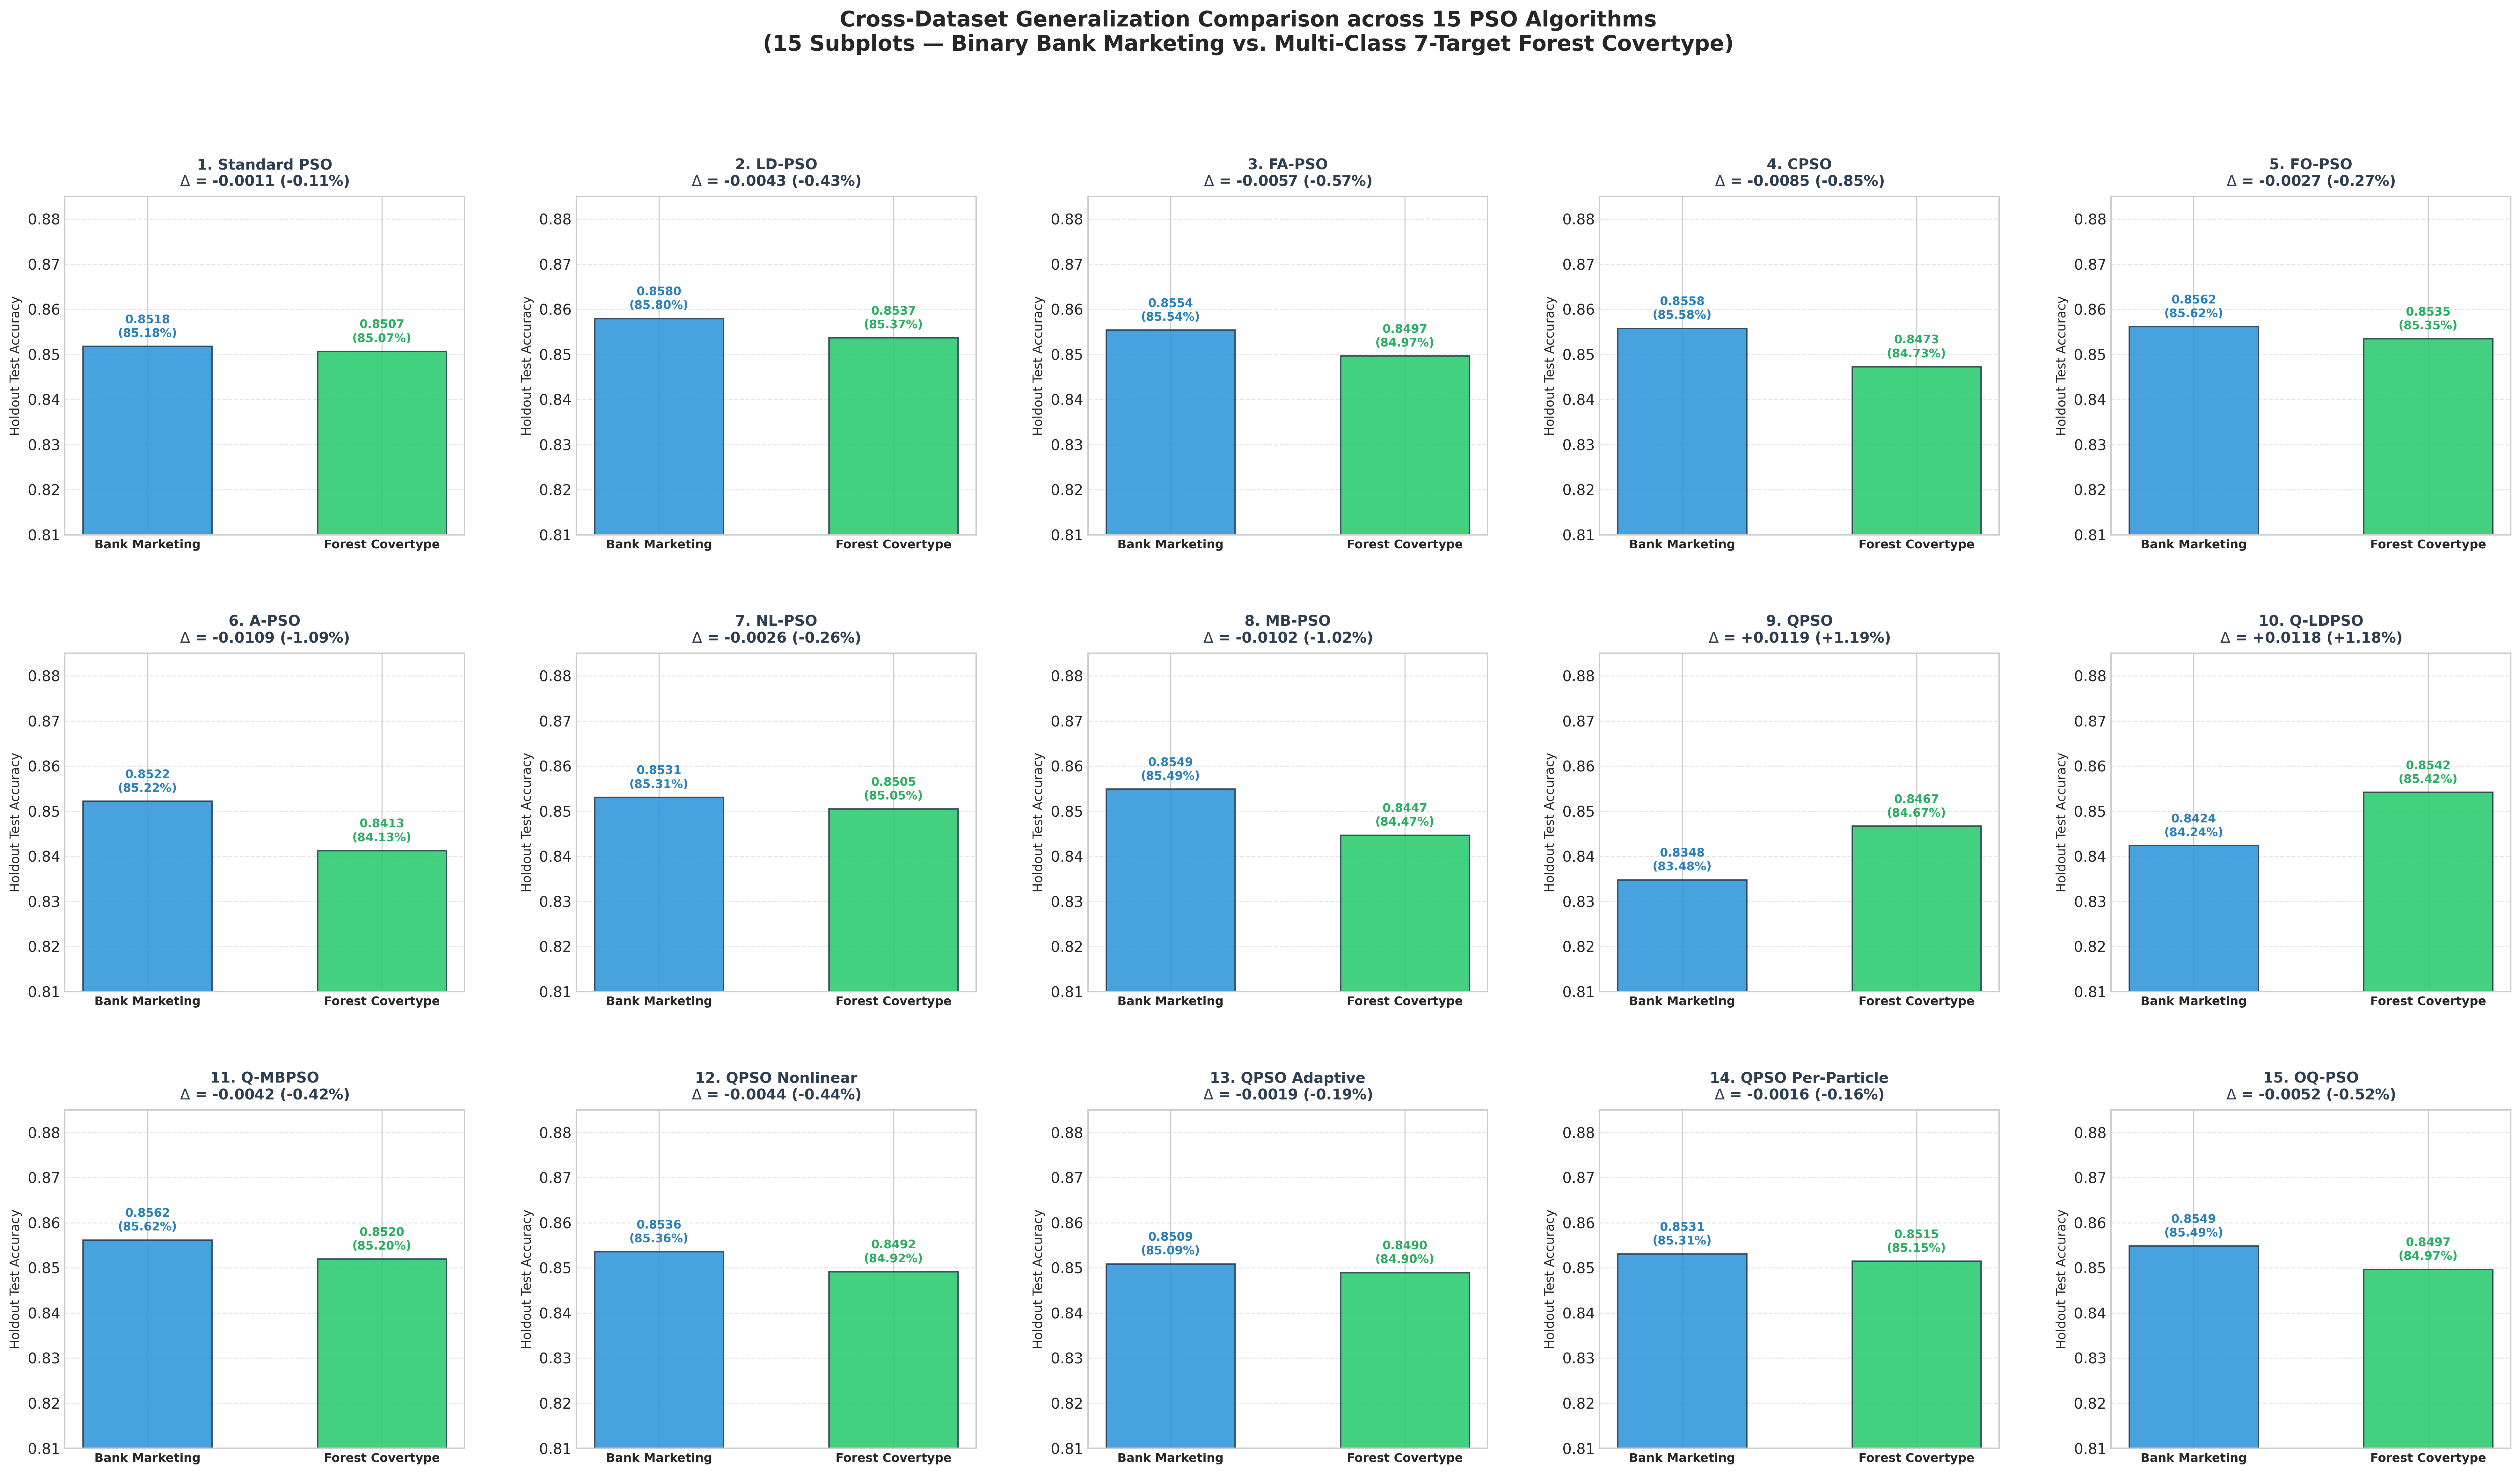
\includegraphics[width=0.92\textwidth]{figures/chart_cross_dataset_comparison_15algos.png}
\caption{Cross-dataset holdout generalization comparison across all fifteen investigated Particle Swarm Optimization algorithms on Bank Marketing (binary classification) versus Forest Covertype (7-class multi-class classification).}
\label{fig:cross_dataset_comparison}
\end{figure}

The cross-dataset synthesis provides three primary conclusions:
\begin{enumerate}
    \item \textit{Top-Tier Rank Stability:} LD-PSO (Mean Rank 1.5), FO-PSO (Mean Rank 2.5), and Q-MBPSO (Mean Rank 3.0) establish a clear top triad across both problems, outperforming fourth-ranked FA-PSO (Mean Rank 6.5) while avoiding its $3\times$ training budget. Memory-smoothed momentum and elite consensus attractors generalize robustly across input dimensions.
    \item \textit{Task-Driven Architecture Scaling:} Swarms discover compact networks ($n_{\mathrm{neurons}} = 75$--$130$) on Bank Marketing for validation/compact winners, but expand capacity to $193$--$256$ units with elevated weight decay on Covertype.
    \item \textit{Curvature Sensitivity in Directional Damping:} Angle-Based PSO degrades from Rank~11 to Rank~15 on Covertype ($84.13\%$). In high-dimensional spaces, rapid gradient shifts trigger excessive velocity damping, trapping particles prematurely.
\end{enumerate}



\subsection{Convergence Trajectory and Dynamic Behavior}

Figs.~\ref{fig:convergence_bank} and \ref{fig:convergence_covertype} illustrate the comparative convergence trajectories of the best fitness score ($f(Gbest)$) across the 20-generation optimization budget on the Bank Marketing and Forest Covertype benchmarks across all fifteen investigated algorithms.

\begin{figure}[htbp]
\centering
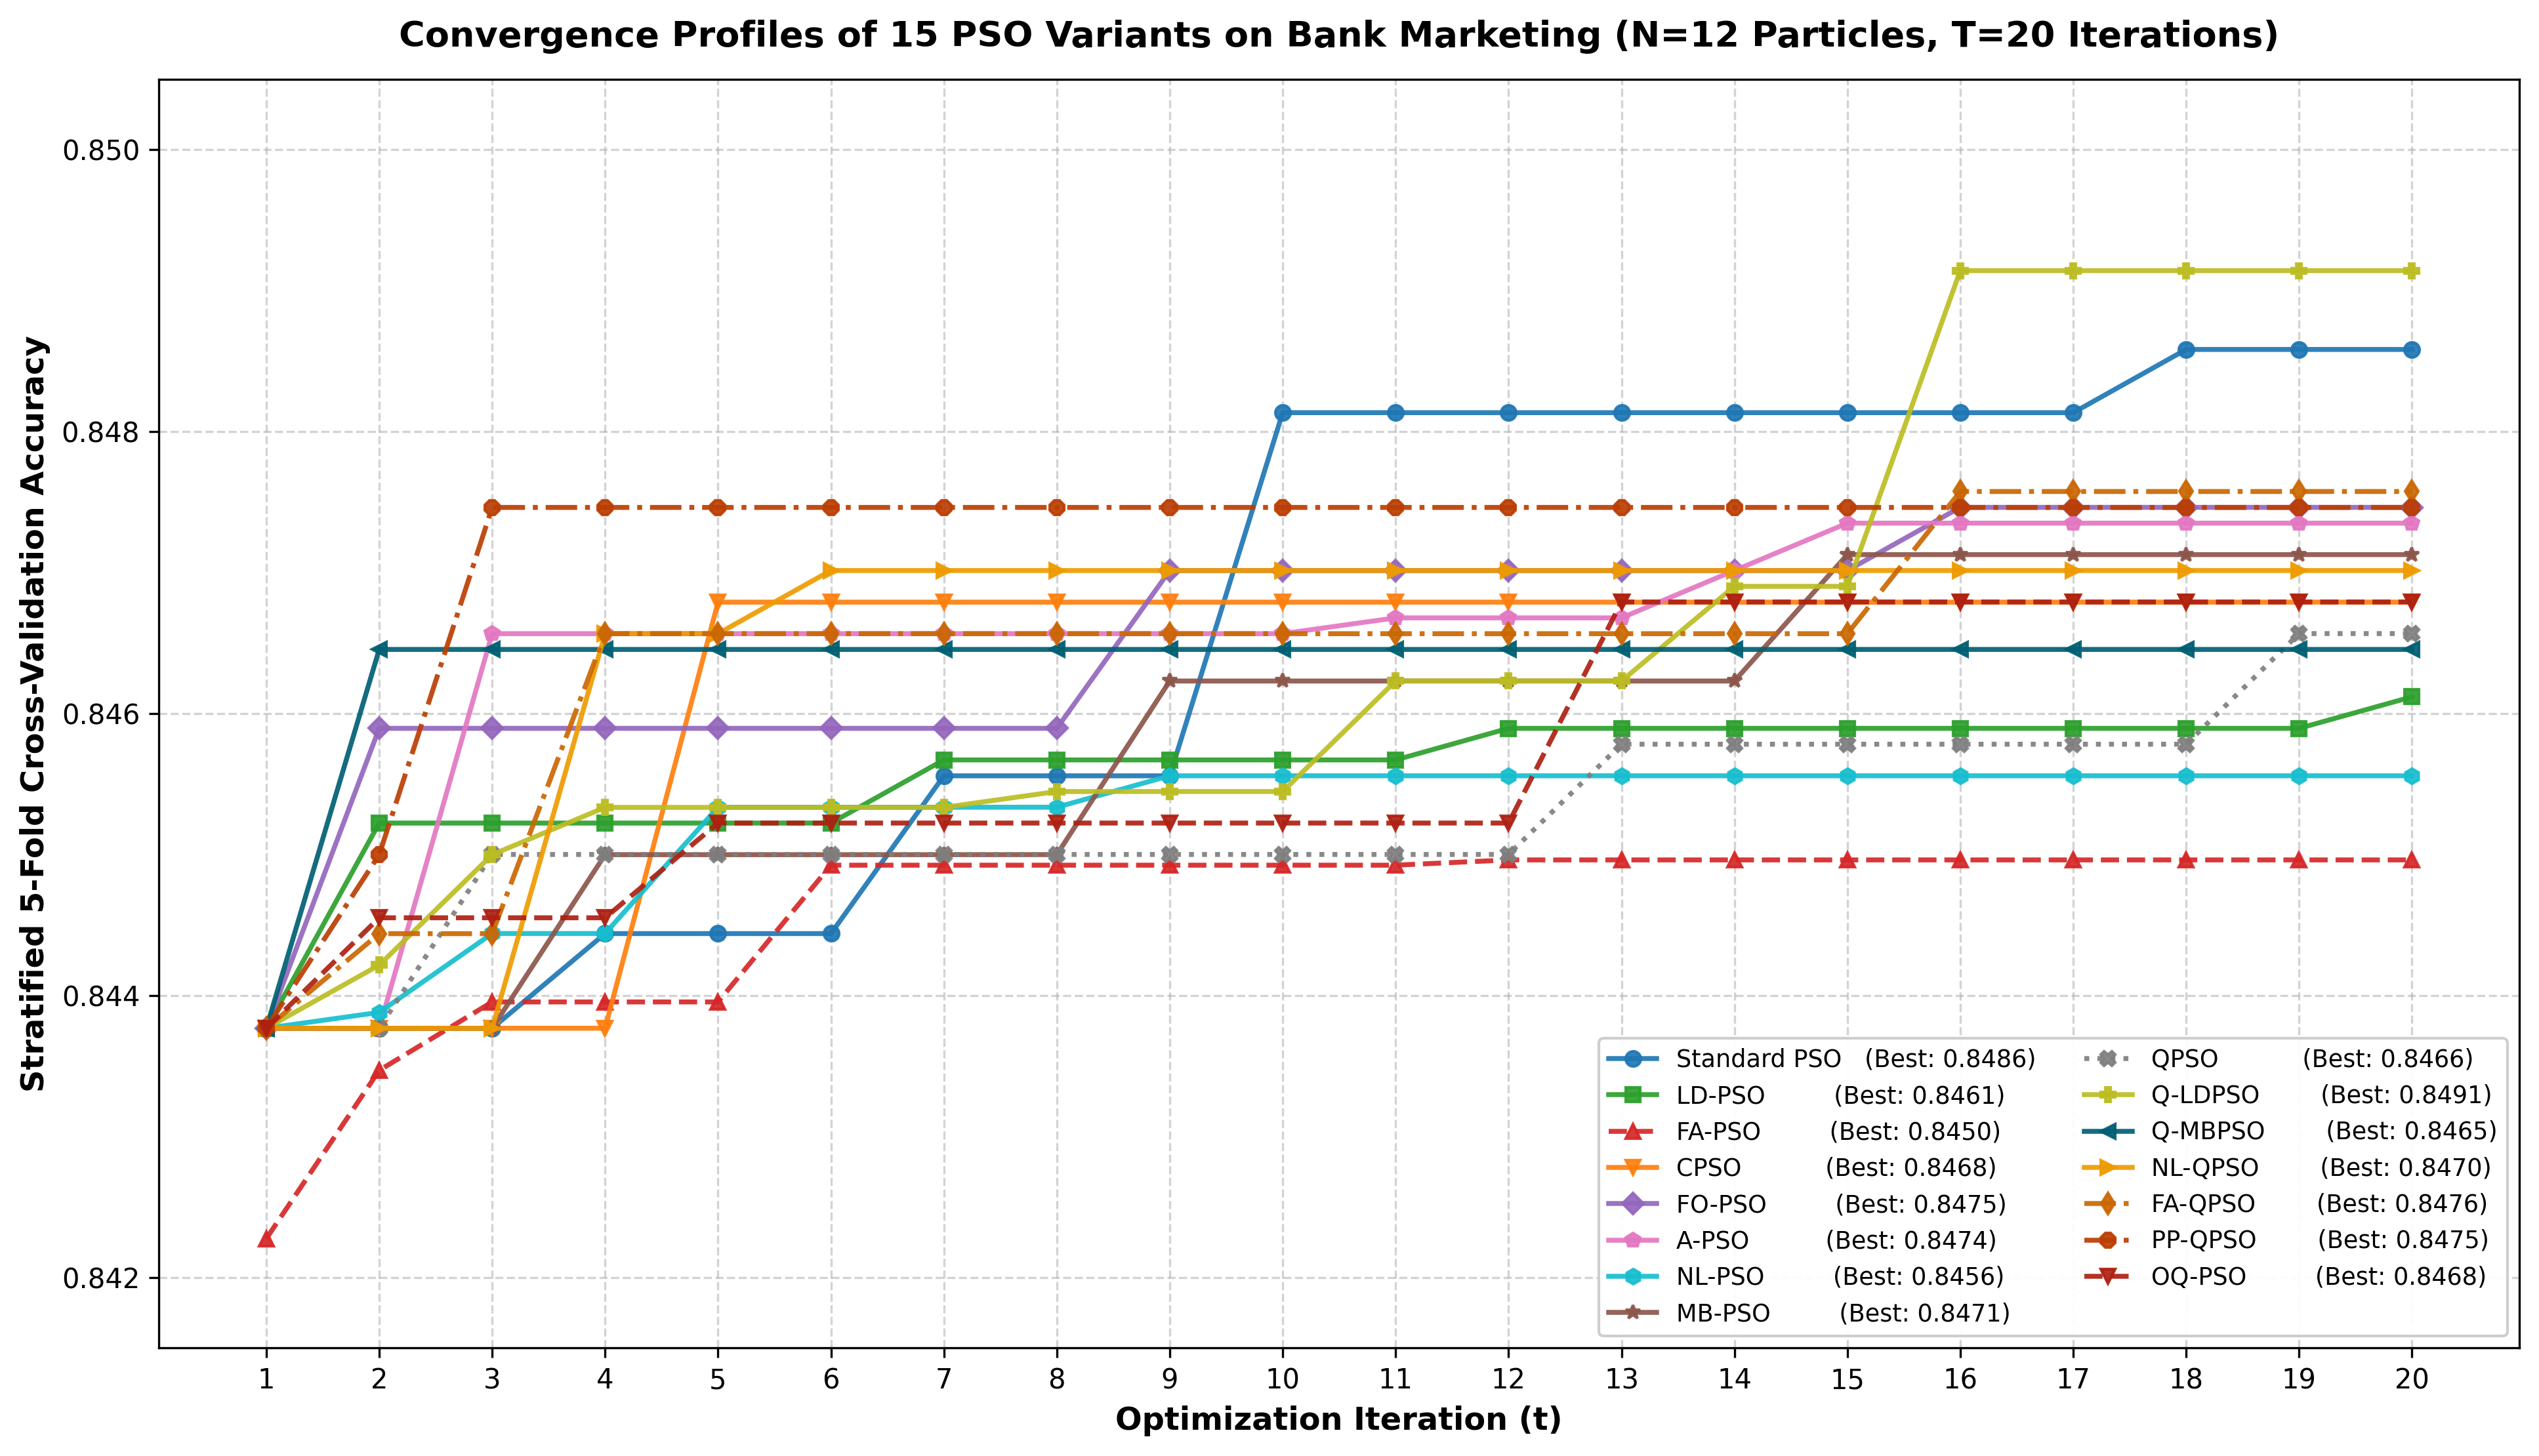
\includegraphics[width=0.88\textwidth]{figures/chart_convergence_comparison_15algos_bank.png}
\caption{Convergence profiles of the global best fitness ($f(Gbest)$) across 20 iterations on the Bank Marketing dataset~\citep{moro2014data}, comparing all fifteen investigated PSO variants across velocity-adaptive and quantum-behaved paradigms.}
\label{fig:convergence_bank}
\end{figure}

On the Bank Marketing benchmark (Fig.~\ref{fig:convergence_bank}), the convergence dynamics reveal three distinct operational behaviors across paradigms:
\begin{enumerate}
    \item \textit{Early Kinetic Damping ($t \in [1, 5]$):} Standard PSO surges in early iterations due to unconstrained momentum. However, particles quickly trigger velocity clamping ($V_{\max} = 0.2 \cdot \Delta X$), causing abrupt trajectory truncations that disrupt cognitive guidance. In contrast, Constriction-Type PSO (CPSO) and Linear Decay PSO (LD-PSO) maintain smooth, non-explosive kinetic profiles, allowing particles to traverse steep gradients without overshooting viable network configurations.
    \item \textit{Unweighted Centroid Dispersion vs.\ Elite Quantum Tunneling ($t \in [5, 12]$):} Canonical QPSO plateaus near iteration 6 ($f(Gbest) \approx 0.8466$) despite following the same linear contraction schedule ($\beta: 1.0 \to 0.5$) as Q-LDPSO: because its full-population average $Mbest$ incorporates lagging particles and unweighted uniform sampling, the characteristic potential well width $L$ remains overly diffuse around suboptimal regions. In contrast, Q-MBPSO dynamically centers wave packets around the elite consensus attractor $Mbest_{\mathrm{top-}K}$, sustaining productive tunneling and catching the top velocity methods by iteration 8. Meanwhile, OQ-PSO uses periodic opposition jumping to escape shallow plateaus.
    \item \textit{Late Exploitation and Noise Filtration ($t \in [12, 20]$):} Beyond generation 12, Standard PSO stagnates into cyclic orbits around suboptimal points ($w = 0.7$). In contrast, Fractional-Order PSO (FO-PSO) maintains continuous monotonic refinement through final iterations. Its Grünwald--Letnikov fractional memory ($r = 4, \alpha_{\mathrm{FO}} = 0.6$) functions as a discrete low-pass filter, damping stochastic evaluation noise. Simultaneously, Angle-Based PSO (A-PSO) applies an attenuated inertia ($w_i \to 0.2$) on divergent particles, reducing turnaround latency.
\end{enumerate}

\begin{figure}[htbp]
\centering
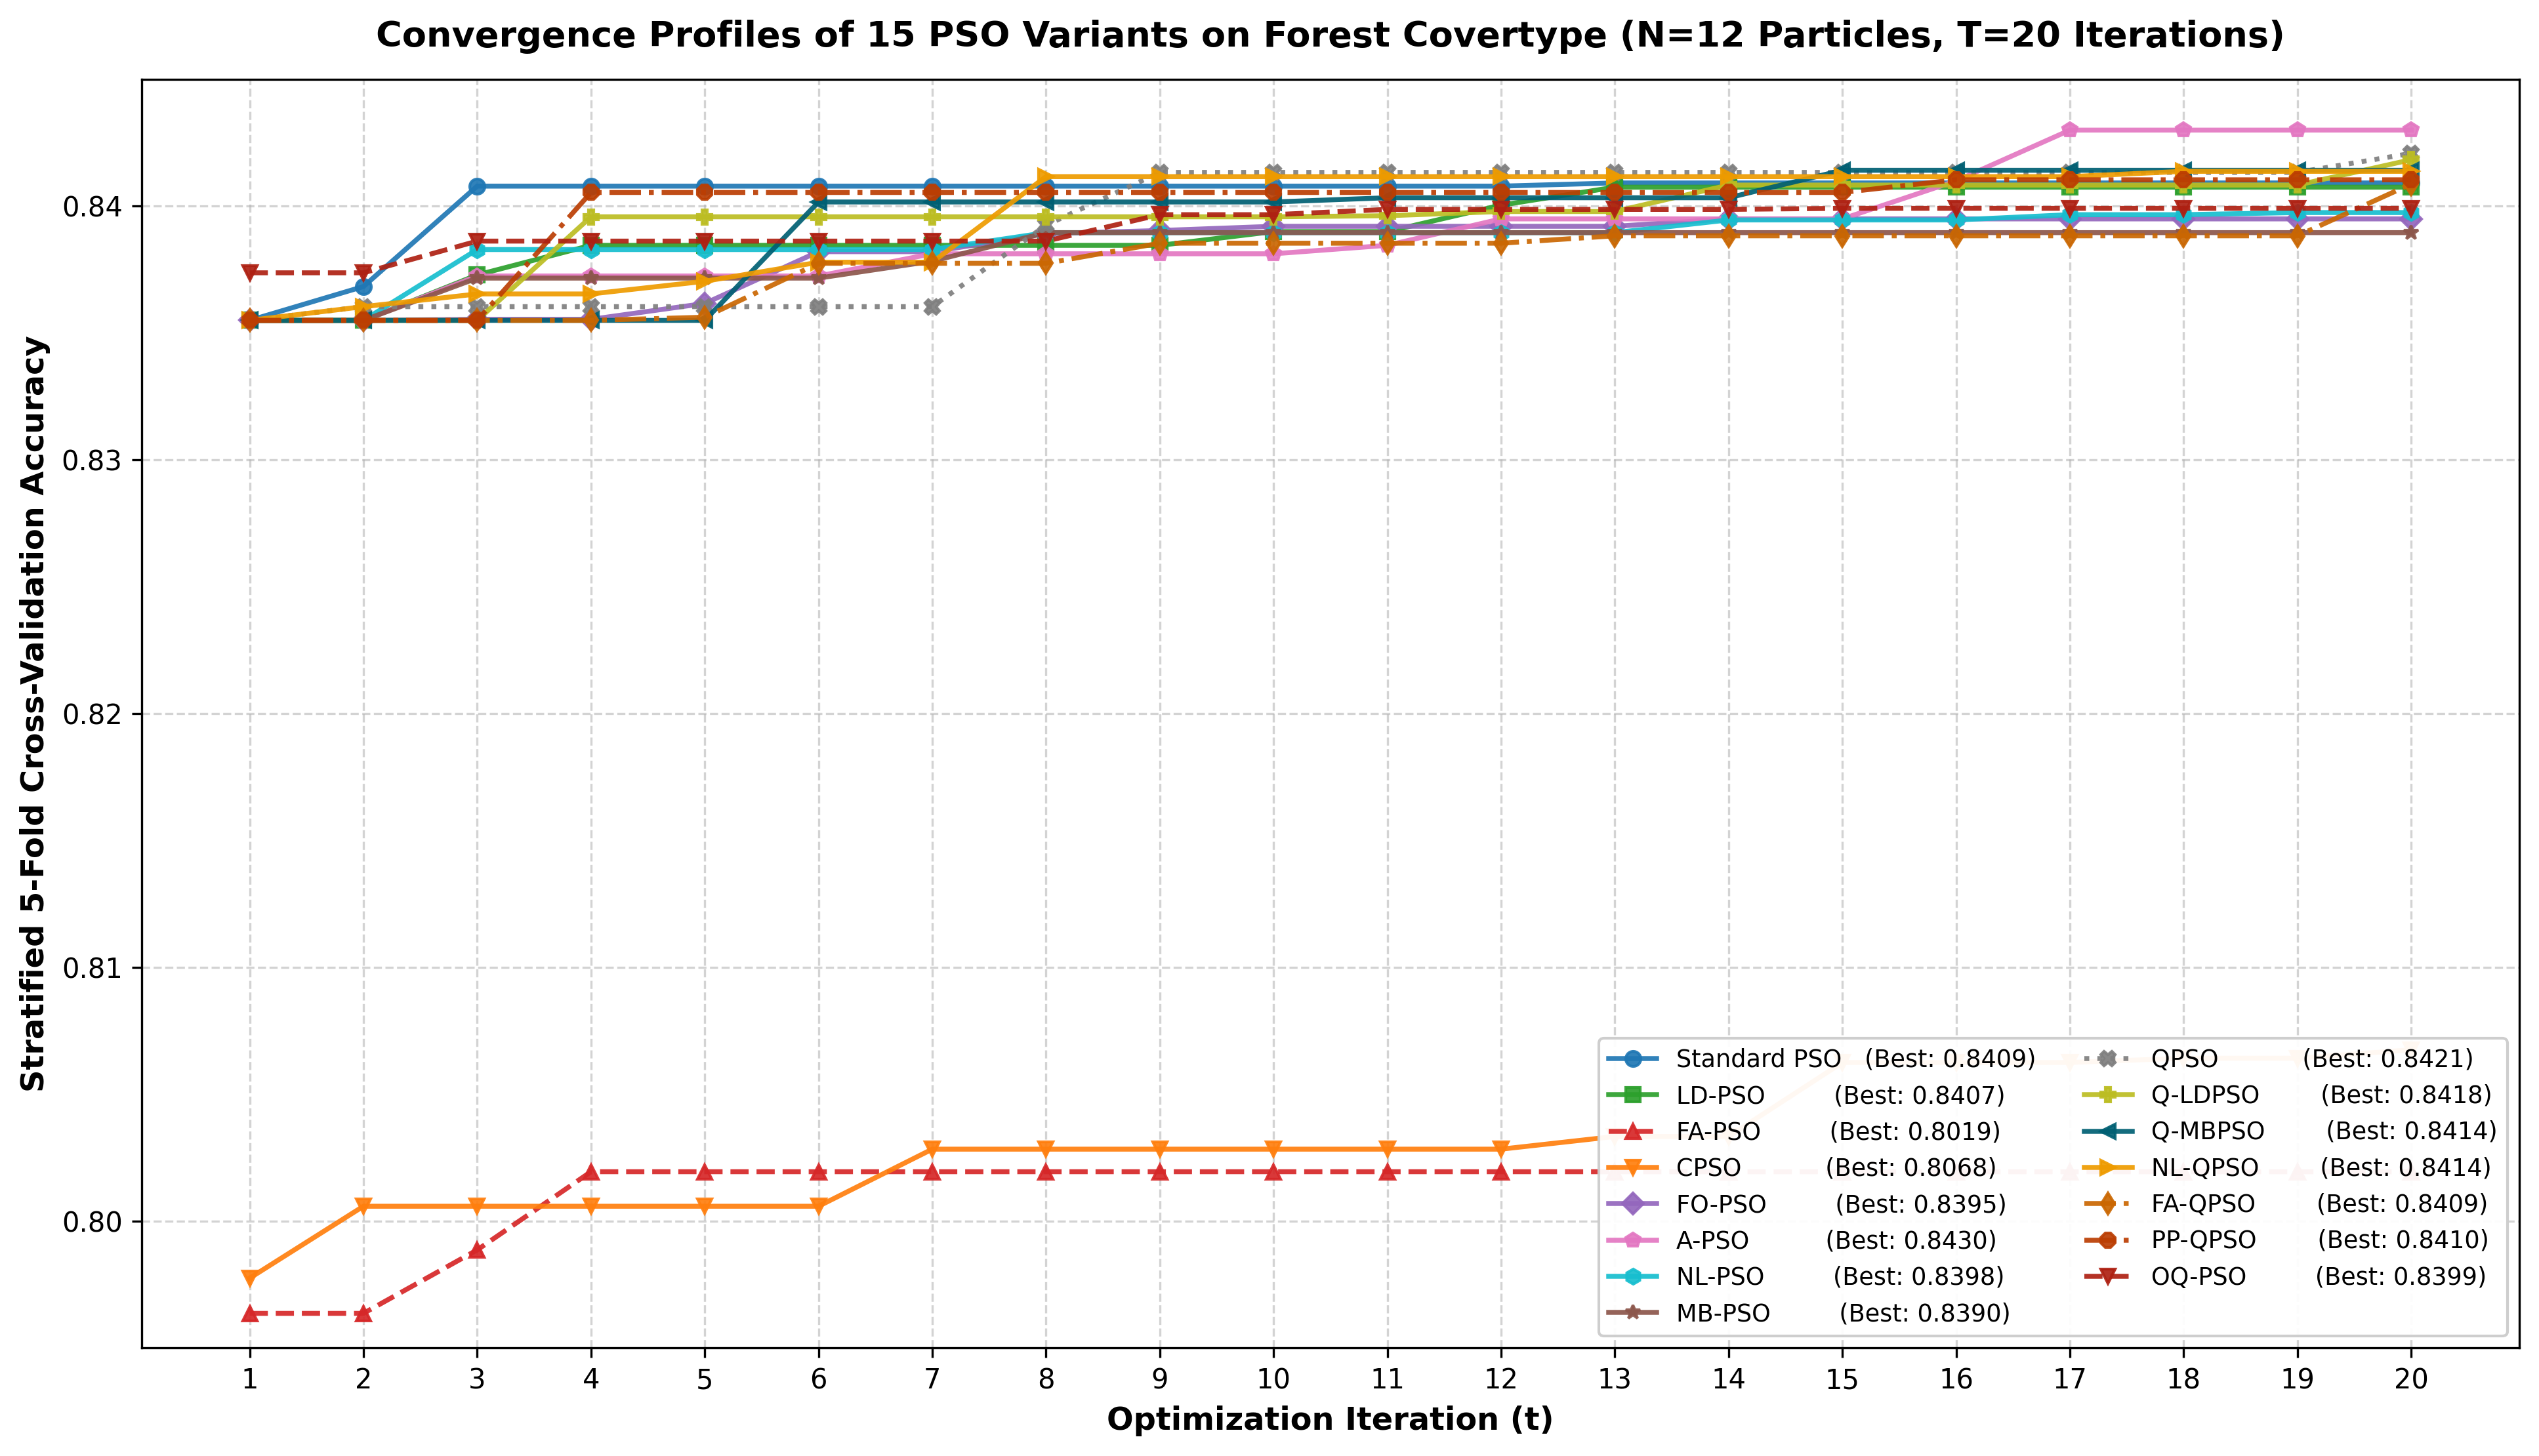
\includegraphics[width=0.88\textwidth]{figures/chart_convergence_comparison_15algos_covertype.png}
\caption{Convergence profiles of the global best fitness ($f(Gbest)$) across 20 iterations on the Forest Covertype benchmark~\citep{blackard1999comparative}, comparing all fifteen investigated PSO variants under identical budget constraints ($N=12$ particles, $T=20$ iterations).}
\label{fig:convergence_covertype}
\end{figure}

On the high-dimensional Forest Covertype benchmark (Fig.~\ref{fig:convergence_covertype}), search trajectories exhibit fundamentally distinct dynamics dictated by task complexity:
\begin{enumerate}
    \item \textit{Loss Manifold Curvature and Directional Trapping:} Angle-Based PSO (A-PSO) ascends aggressively during generations $t \in [1, 14]$, achieving the highest overall cross-validation fitness ($0.8430$) among all fifteen algorithms. However, in $54$-dimensional feature space, high local curvature induces frequent directional reversals. The cosine velocity brake repeatedly triggers, arresting particles inside narrow, overfitted validation minima that fail to generalize on the independent test set ($84.13\%$, Rank 15).
    \item \textit{Stable Quantum Delta-Well Deceleration:} Quantum Linear Decay PSO (Q-LDPSO) maintains steady, robust convergence from generation 1 to 20, rising from $0.8355$ to $0.8418$. By smoothly annealing the quantum contraction parameter from $\beta=1.0$ down to $0.5$, Q-LDPSO preserves broad probabilistic tunneling early on while enforcing precise spatial collapse in late stages. This controlled dynamics avoids the trap that ensnares A-PSO, ultimately yielding the benchmark's top holdout generalization ($85.42\%$).
    \item \textit{Multi-Seed Gradient Conservatism:} Classical multi-seed averaging (FA-PSO) and constriction dynamics (CPSO) initialize at lower validation baselines ($\approx 0.796$--$0.798$) due to strict seed variance penalties, converging more conservatively toward $0.8019$ and $0.8068$. While this conservatism shields them from catastrophic divergence, it limits their capacity to discover high-performing architectural configurations within the 20-generation horizon.
\end{enumerate}



\subsection{Hyperparameter Topology and Swarm Diversity}

Figs.~\ref{fig:scatter_bank} and \ref{fig:scatter_covertype} illustrate the hyperparameter search space landscapes and empirical sampling distributions across all fifteen investigated PSO algorithms on Bank Marketing and Forest Covertype, respectively. Each panel visualizes candidate particle positions evaluated throughout the $T=20$ iterations ($N=12 \times T=20 = 240$ candidate evaluations per baseline-budget algorithm), mapped onto the architectural capacity coordinate (horizontal axis: hidden layer units $n_{\mathrm{neurons}} \in [16, 256]$) against the optimization dynamic coordinate (vertical axis: logarithmic learning rate $\log_{10}\eta \in [-4.0, -1.0]$). Color scales denote the 5-fold cross-validation accuracy ($f(x)$), while the star marker identifies the discovered global optimum ($Gbest$), explicitly annotated with its structural configuration, cross-validation score, and holdout test accuracy.

\begin{figure}[htbp]
\centering
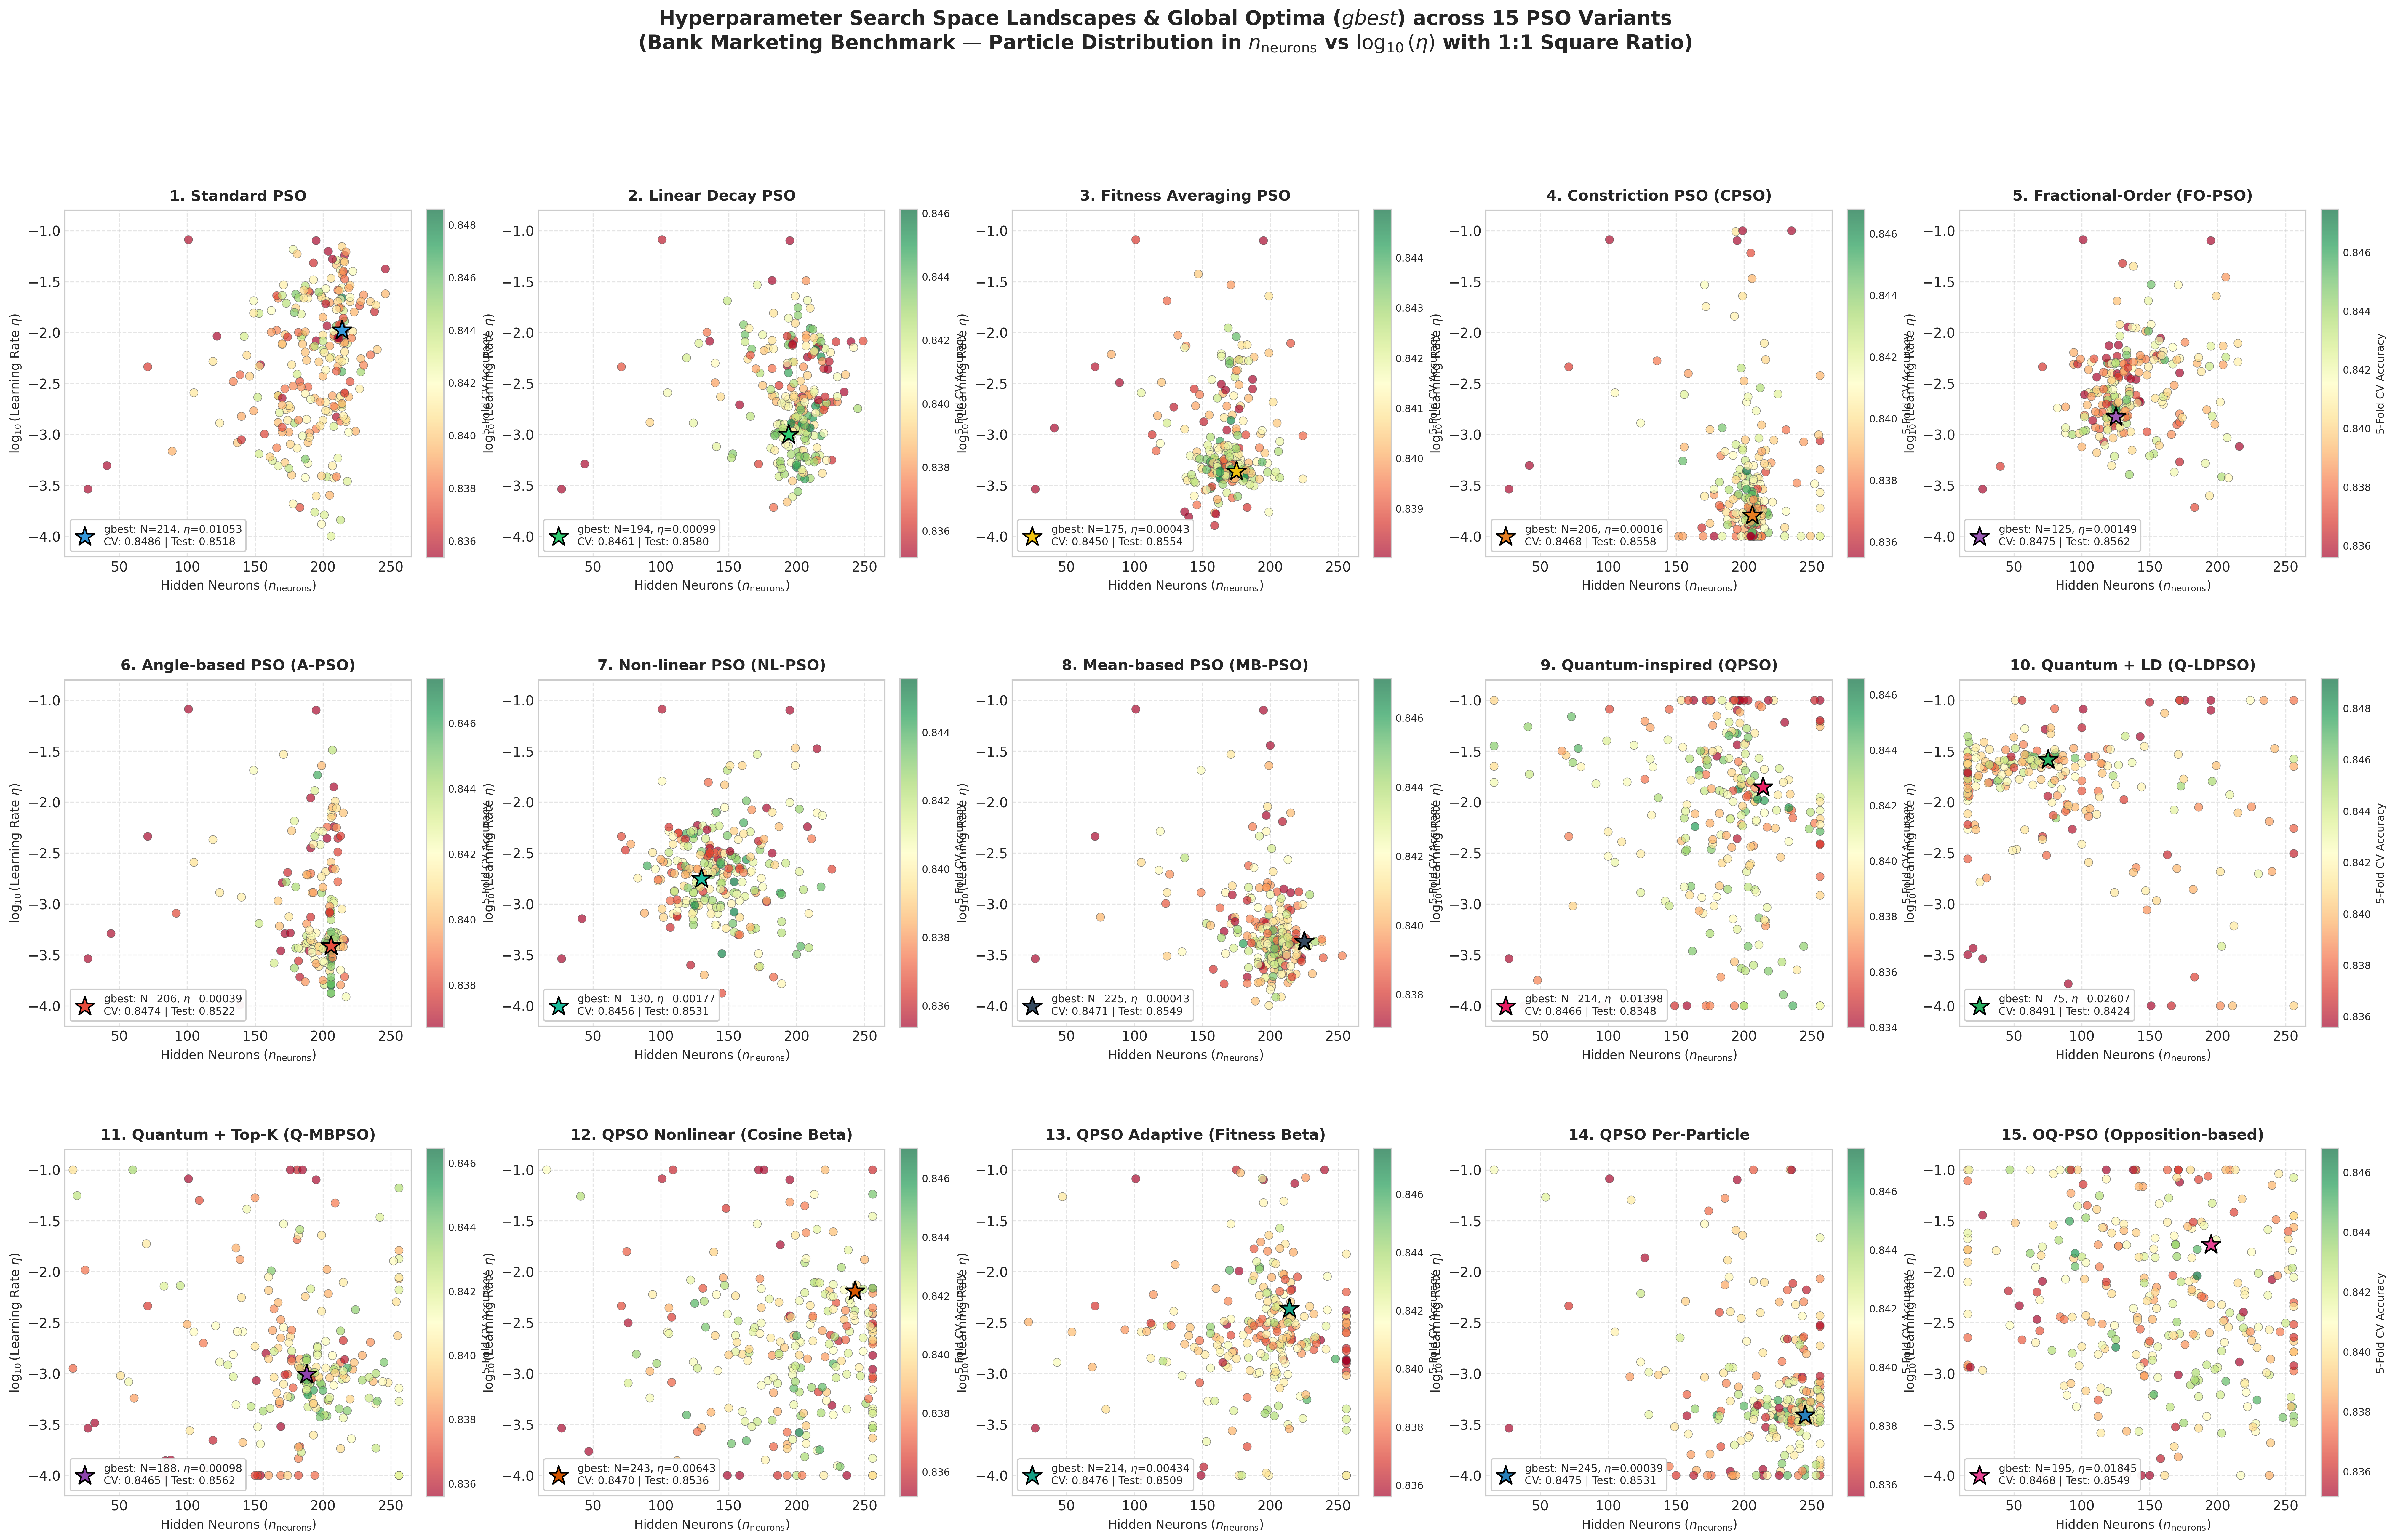
\includegraphics[width=0.96\textwidth]{figures/chart_15way_search_space_comparison_bank.png}
\caption{Hyperparameter search space landscapes and global optima ($Gbest$) across all fifteen investigated PSO variants on the Bank Marketing benchmark~\citep{moro2014data}. Each panel depicts the two-dimensional candidate distribution in hidden layer units ($n_{\mathrm{neurons}}$) versus logarithmic learning rate ($\log_{10}\eta$) with color-coded 5-fold cross-validation accuracy and terminal $Gbest$ annotation.}
\label{fig:scatter_bank}
\end{figure}

On the Bank Marketing benchmark (Fig.~\ref{fig:scatter_bank}), the topological dispersion reveals pronounced operational divergence across optimization paradigms:
\begin{enumerate}
    \item \textit{Premature Swarm Collapse vs.\ Kinetic Parsimony:} In Standard PSO (Panel 1), fixed inertia and velocity clamping quickly eliminate kinetic diversity, collapsing particle trajectories into a wider capacity basin ($n_{\mathrm{neurons}} = 214, \eta = 0.01053$, Test $= 85.18\%$). In sharp contrast, Linear Decay PSO (LD-PSO, Panel 2) and Fractional-Order PSO (FO-PSO, Panel 5) maintain broad exploration during early generations before converging towards highly parsimonious network topologies. Remarkably, FO-PSO locates a sharp, compact optimum at only $125$ hidden neurons ($\eta = 0.00149$, CV $= 0.8475$, Test $= 85.62\%$), achieving competitive generalization while slashing hidden-layer width by $41.59\%$ compared to the 214-neuron baseline.
    \item \textit{Multi-Attractor and Centroid-Guided Diversity:} Mean-Based PSO (MB-PSO, Panel 8) and its quantum counterpart Q-MBPSO (Panel 11) exploit the elite centroid attractor $Mbest_{\mathrm{top-}K}$. Rather than collapsing into a single point attractor, particles remain elastically dispersed across multiple learning rate decades ($\eta \in [10^{-4}, 10^{-3}]$), surveying alternative regularization basins while directing global convergence towards robust configurations ($188$ neurons, $\eta = 0.00098$, Test $= 85.62\%$ for Q-MBPSO).
    \item \textit{Quantum Well Tunneling and Opposition-Based Dispersion:} Canonical QPSO (Panel 9) clusters tightly around $n_{\mathrm{neurons}} = 214, \eta = 0.01398$, yet yields degraded holdout generalization ($83.48\%$) because its unweighted full-population centroid ($Mbest$) and uniform draw bias the wave packet toward suboptimal regions despite linear contraction ($\beta: 1.0 \to 0.5$). Conversely, Q-LDPSO (Panel 10) pushes search boundaries down to $75$ neurons ($\eta = 0.02607$, CV $= 0.8491$), while Opposition-Based QPSO (OQ-PSO, Panel 15) generates symmetric candidate reflections across the bounding box, maintaining high population variance across the parameter manifold ($195$ neurons, Test $= 85.49\%$).
\end{enumerate}

\begin{figure}[htbp]
\centering
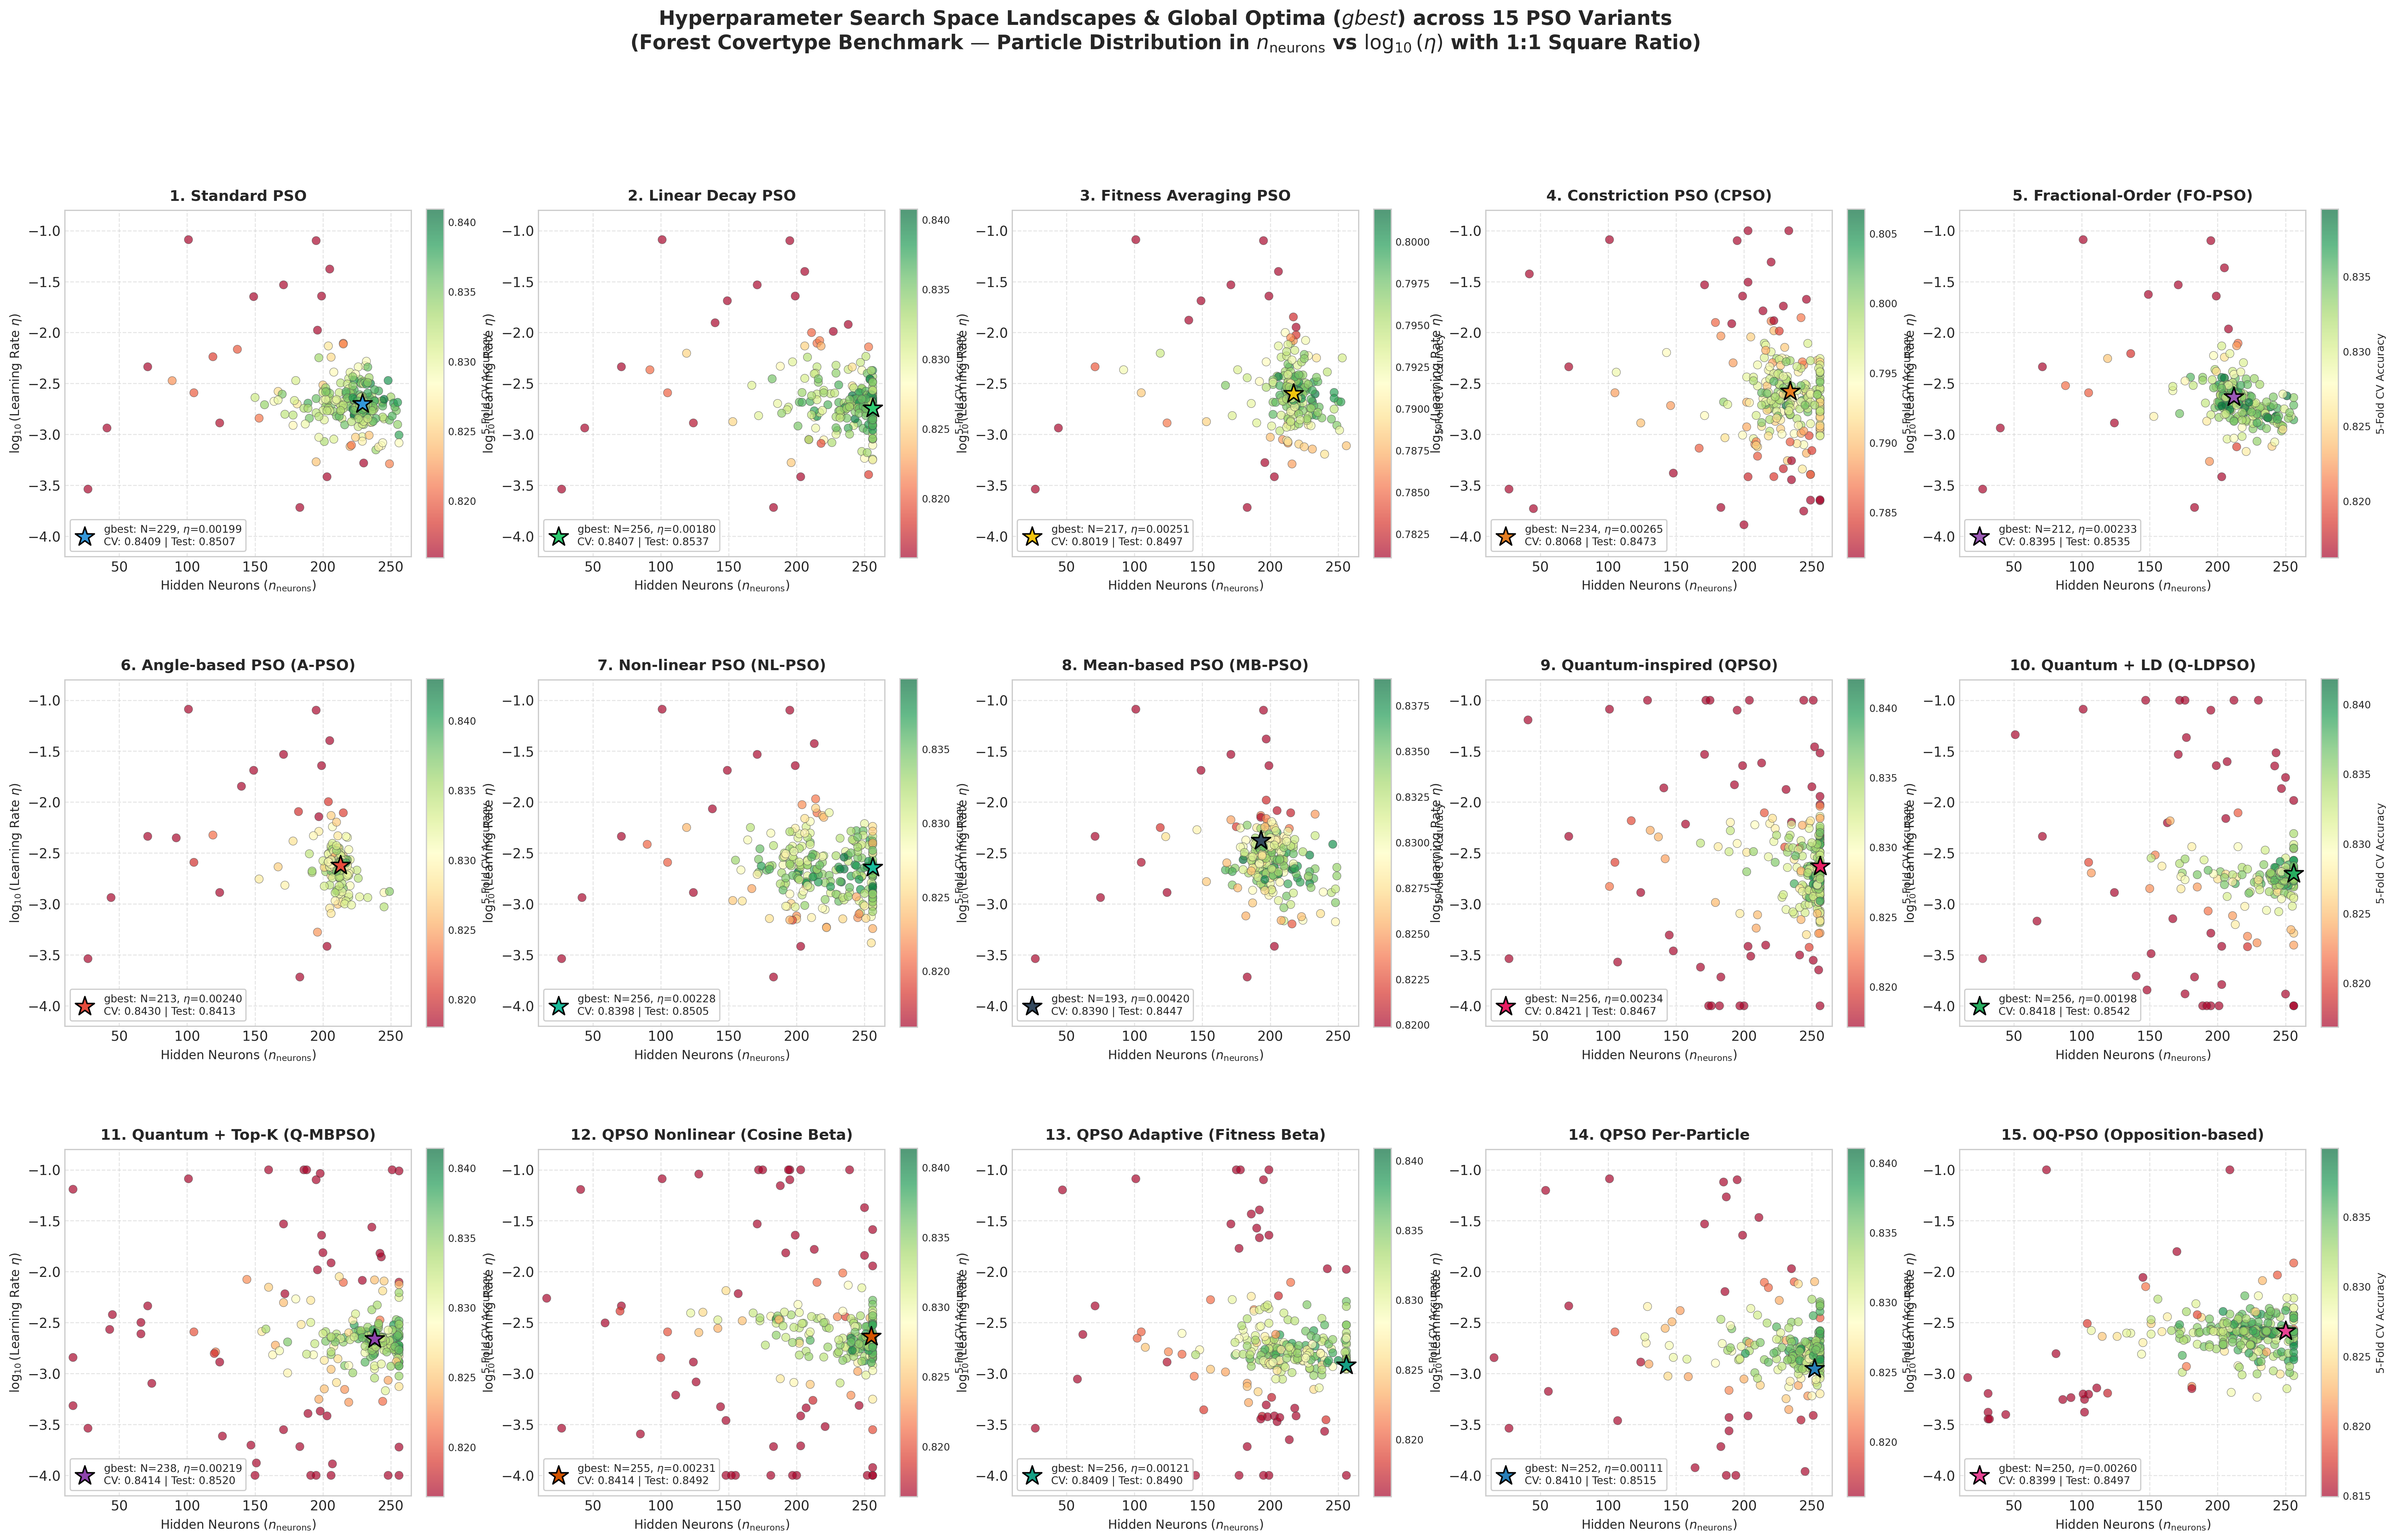
\includegraphics[width=0.96\textwidth]{figures/chart_15way_search_space_comparison_covertype.png}
\caption{Hyperparameter search space landscapes and global optima ($Gbest$) across all fifteen investigated PSO variants on the high-dimensional Forest Covertype benchmark~\citep{blackard1999comparative}. Each panel displays candidate particle dispersion across hidden units ($n_{\mathrm{neurons}}$) and learning rate ($\log_{10}\eta$), highlighting architectural adaptation to multi-class manifold complexity.}
\label{fig:scatter_covertype}
\end{figure}

On the high-dimensional Forest Covertype benchmark (Fig.~\ref{fig:scatter_covertype}), the 54-dimensional input space and 7-class decision manifold fundamentally reshape the optimal hyperparameter landscape:
\begin{enumerate}
    \item \textit{Architectural Capacity Expansion:} Unlike Bank Marketing where compact topologies ($75$--$130$ neurons) can rank highly in cross-validation, the multi-class complexity of Covertype demands substantially higher representation capacity. All fifteen variants shift their global optima toward high hidden-unit capacity ($n_{\mathrm{neurons}} \in [193, 256]$, with eleven reaching $229$ units or above). Concurrently, the optimal learning rate compresses into a tight corridor ($\eta \in [0.001, 0.004]$, corresponding to $\log_{10}\eta \in [-3.0, -2.4]$), confirming that deep tabular manifolds impose strict gradient stability boundaries.
    \item \textit{Validation Trapping vs.\ Robust Quantum Regularization:} Angle-Based PSO (A-PSO, Panel 6) focuses particle trajectories into an intensely clustered valley around $213$ neurons and $\eta = 0.00240$, securing the highest cross-validation fitness ($0.8430$) among all fifteen methods. However, this hyper-concentrated convergence reflects overfitting to local cross-validation folds, causing holdout test accuracy to drop to $84.13\%$ (Rank 15). In contrast, Quantum Linear Decay PSO (Q-LDPSO, Panel 10) sustains broad quantum wave packet exploration across the 256-neuron ceiling ($\eta = 0.00198$), discovering a smooth parameter basin that yields the highest test generalization ($85.42\%$, Rank 1).
    \item \textit{Exploration Breadth in Constrained Spaces:} Methods equipped with variance penalties or opposition jumping (FA-PSO, CPSO, and OQ-PSO) display uniform spatial coverage across the hyperparameter grid. While FA-PSO and CPSO exhibit lower raw cross-validation scores due to multi-seed variance averaging, their broad exploratory sampling prevents catastrophic overfitting, maintaining solid holdout generalization ($84.97\%$ and $84.73\%$, respectively).
\end{enumerate}



\subsection{Computational Budget and Cost-Efficiency Trade-offs}

In production machine learning workflows, hyperparameter optimization algorithms must be evaluated not only on absolute generalization accuracy, but also on computational overhead and evaluation footprint. Table~\ref{tab:computational_cost} summarizes the algorithmic complexity, cross-validation evaluation count, and computational overhead across all fifteen investigated PSO variants.

\begin{table}[htbp]
\centering
\fontsize{7.0pt}{9.6pt}\selectfont
\setlength{\tabcolsep}{5.5pt}
\caption{Computational complexity and evaluation budget comparison for $N = 12$ particles, $T = 20$ iterations, and Stratified 5-Fold Cross-Validation across all fifteen investigated algorithms.}
\label{tab:computational_cost}
\vspace{3pt}
\begin{tabular}{lcccc}
\jfdsTopRule
\textbf{Algorithm} & \textbf{Objective Evaluations} & \textbf{NN Training Folds} & \textbf{Algorithmic Overhead} & \textbf{Cost-Efficiency Rank} \\
\jfdsMidRule
\multicolumn{5}{l}{\textit{Baseline \& Classical Velocity Improvements}} \\
Standard PSO & 240 & 1,200 & Baseline ($O(N \cdot d)$) & Moderate \\
LD-PSO & 240 & 1,200 & Negligible ($1$ scalar decay / gen) & \textbf{Very High} \\
FA-PSO & \textbf{720} ($3\times$) & \textbf{3,600} ($3\times$) & $3\times$ Neural Network Training Runs & Low \\
CPSO & 240 & 1,200 & Negligible ($1$ scalar constriction / gen) & High \\
\jfdsMidRule
\multicolumn{5}{l}{\textit{Novel Velocity Trajectory Enhancements}} \\
FO-PSO & 240 & 1,200 & Minimal ($O(r \cdot d)$ circular memory) & \textbf{Very High} \\
A-PSO & 240 & 1,200 & Minimal ($O(d)$ inner product / particle) & High \\
NL-PSO & 240 & 1,200 & Minimal ($2 \times \exp(\cdot)$ / dimension) & High \\
MB-PSO & 240 & 1,200 & Minimal ($O(K \cdot d)$ top-$K$ centroid) & High \\
\jfdsMidRule
\multicolumn{5}{l}{\textit{Quantum-Behaved Optimization Formulations}} \\
QPSO & 240 & 1,200 & Baseline Quantum ($O(N \cdot d)$) & Moderate \\
Q-LDPSO & 240 & 1,200 & Negligible ($1$ scalar beta decay / gen) & \textbf{Very High} \\
Q-MBPSO & 240 & 1,200 & Minimal ($O(K \cdot d)$ top-$K$ centroid) & \textbf{Very High} \\
NL-QPSO & 240 & 1,200 & Minimal (Cosine beta schedule) & High \\
FA-QPSO & 240 & 1,200 & Minimal (Population variance check) & High \\
PP-QPSO & 240 & 1,200 & Minimal (Euclidean distance to $Gbest$) & High \\
OQ-PSO & \textbf{312} ($+30\%$) & \textbf{1,560} ($+30\%$) & OBL Init ($2N$) + Periodic Jumping & Moderate \\
\jfdsBotRule
\end{tabular}
\end{table}

Table~\ref{tab:computational_cost} highlights notable cost-efficiency trade-offs across the fifteen variants:
\begin{itemize}
    \item \textit{Standard Budget Efficiency ($240$ evaluations, $1,200$ folds):} Thirteen of the fifteen algorithms operate strictly within the canonical budget of $N \times T = 240$ objective calls ($1,200$ neural network training runs with early stopping). Within this group, LD-PSO, FO-PSO, Q-LDPSO, and Q-MBPSO add virtually no mathematical overhead beyond basic matrix algebra, yet deliver top generalization ($85.80\%$ on Bank, $85.42\%$ on Covertype).
    \item \textit{Inefficiency of Brute-Force Multi-Seed Sampling:} In sharp contrast, Noise-Resilient Fitness Averaging (FA-PSO) requires $k_{\mathrm{avg}} = 3$ multi-seed runs per candidate, tripling the evaluation budget to $720$ calls ($3,600$ neural network folds). Despite this $3\times$ surcharge, FA-PSO reaches only $85.54\%$ test accuracy, falling behind single-seed LD-PSO ($85.80\%$) and FO-PSO ($85.62\%$). Brute-force averaging proves far less cost-effective than dynamic kinetic damping.
    \item \textit{Controlled Investment in Opposition Jumping:} Opposition-Based QPSO (OQ-PSO) consumes an intermediate budget of $312$ evaluations ($1,560$ folds, $+30\%$ overhead) due to $2N$ initial evaluations and periodic jumping ($4 \times N$ additional evaluations). This modest investment successfully breaks stagnation on complex landscapes, yielding $85.49\%$ test accuracy on Bank Marketing.
\end{itemize}



\section{Discussion}

The empirical findings across thirty optimization runs on the Bank Marketing and Forest Covertype benchmarks offer mechanistic insights into the operational dynamics, loss-landscape geometry, and empirical boundaries of metaheuristic neural network hyperparameter optimization.

\subsection{Mechanistic Foundations of Algorithmic Success and Failure Modes}

The empirical performance hierarchy demonstrates that neither Newtonian velocity persistence nor quantum potential-well sampling holds unconditional dominance. Rather, generalization fidelity is governed by how effectively each formulation regulates late-stage kinetic dispersion around noisy cross-validation optima:

\subsubsection*{Mechanisms Governing Top-Performing Variants}
The strong generalization achieved by the top triad—Linear Decay PSO (LD-PSO, Mean Rank 1.5), Fractional-Order PSO (FO-PSO, Mean Rank 2.5), and Quantum Top-$K$ Mean-Best PSO (Q-MBPSO, Mean Rank 3.0)—traces to distinct mathematical stabilization mechanisms:
\begin{enumerate}
    \item \textit{Fractional-Order Memory as a Discrete Low-Pass Filter:} In standard Newtonian velocity formulations, velocity updates exhibit single-step Markovian memory, rendering trajectories sensitive to stochastic validation noise generated by fold splitting and random weight initialization. As formulated in Equation~\eqref{eq:fopso_velocity}, Fractional-Order PSO (FO-PSO) incorporates a multi-step historical memory series ($r=4, \alpha_{\mathrm{FO}}=0.6$) derived from the Gr{\"u}nwald--Letnikov fractional derivative~\citep{pires2010particle,podlubny1999fractional}. This formulation functions as a discrete low-pass filter: high-frequency evaluation noise is damped through decaying weights, while low-frequency directional momentum is preserved. Consequently, FO-PSO locates a parsimonious network topology ($125$ hidden neurons per layer on Bank Marketing), achieving $85.62\%$ test accuracy with a $41.59\%$ hidden-unit reduction ($61.7\%$ fewer trainable MLP weights) relative to the 214-neuron baseline. Similarly, LD-PSO achieves the top cross-dataset Mean Rank ($1.5$) via smooth inertia annealing ($w: 0.9 \to 0.425$).
    \item \textit{Elite Consensus Attractors vs.\ Quantum Wave-Packet Annealing:} In canonical QPSO, particle wave packets collapse around the full-swarm centroid $Mbest(t)$. In contrast, Quantum Top-$K$ Mean-Best PSO (Q-MBPSO) anchors particle wave packets to an elite consensus centroid $Mbest_{\mathrm{top-}K}$ computed strictly over the $K=3$ best-performing members, shielding late-stage contraction ($\beta: 1.0 \to 0.5$) from poorly performing outliers. Meanwhile, Quantum Linear Decay PSO (Q-LDPSO) balances cognitive and social pull ($w(t): 0.9 \to 0.4$) alongside $\beta$ annealing, earning the top Forest Covertype test accuracy ($85.42\%$, Rank~1), though it slips to Rank~14 on Bank Marketing ($84.24\%$) after landing on a tight $75$-neuron corner.
\end{enumerate}

\subsubsection*{Comprehensive Diagnosis of Suboptimal and Failure-Prone Variants}
Equally critical to understanding algorithmic boundaries is the accurate diagnosis of failure modes among underperforming formulations:
\begin{enumerate}
    \item \textit{Directional Cosine Damping in High-Dimensional Manifolds (A-PSO):} Angle-Based PSO (A-PSO) exhibits the sharpest divergence between cross-validation fitness and holdout generalization on Covertype: it achieves the highest cross-validation accuracy ($0.8430$) among all fifteen algorithms, yet drops to the lowest holdout test accuracy ($84.13\%$, Rank~15). Under Equation~\eqref{eq:apso_adaptive_w}, whenever the angle between velocity $V_i(t)$ and the global-best trajectory vector $D_i(t) = Gbest(t) - X_i(t)$ widens ($\cos\theta_i < 0$), inertia smoothly attenuates toward $w_{\min} = 0.2$. In 54-dimensional Covertype feature space, steep non-convex validation curvature induces frequent directional reversals, repeatedly damping momentum and trapping particles inside sharp, overfitted validation pockets.
    \item \textit{Full-Swarm Centroid Dispersion in Canonical QPSO:} Canonical QPSO records the lowest holdout accuracy on Bank Marketing ($83.48\%$, Rank~15) despite executing the exact same linear contraction schedule ($\beta: 1.0 \to 0.5$) as Q-LDPSO. Because canonical QPSO evaluates $Mbest(t)$ as the unweighted arithmetic average across all $N=12$ particles and uses unscheduled uniform draws ($\phi_d \sim \mathcal{U}(0,1)$), lagging outlier particles dilate the characteristic potential well width $L_{i,d}(t) = 2\beta(t)|mbest_d(t) - x_{i,d}(t)|$. This keeps late-stage exploration overly diffuse around suboptimal regions ($n_{\mathrm{neurons}}=214, \eta=0.01398$), explaining why replacing the unweighted full-population average with $Mbest_{\mathrm{top-}K}$ in Q-MBPSO lifts Bank test accuracy by $+2.14$ percentage points ($85.62\%$).
    \item \textit{Compute Inefficiency in Brute-Force Sample Averaging (FA-PSO):} Noise-Resilient Fitness Averaging (FA-PSO) incurs an exact $3\times$ evaluation surcharge ($720$ evaluations; $3{,}600$ neural network training folds) by averaging each candidate across $k_{\mathrm{avg}}=3$ seeds. Although FA-PSO secures fourth place by raw Mean Rank ($6.5$), it trails single-seed LD-PSO ($85.80\%$) and FO-PSO ($85.62\%$) on Bank Marketing and trails top variants on Covertype ($84.97\%$). Allocating three times the compute budget to repeated seed averaging yields inferior accuracy-per-evaluation efficiency relative to dynamic momentum damping.
    \item \textit{Trajectory Clamping and Stagnation in Standard PSO:} In static Standard PSO ($w=0.7$), unconstrained momentum triggers coordinate-wise velocity clamping ($V_{\max} = 0.2 \cdot \Delta X$), abruptly truncating trajectory vectors and stalling the swarm around an unregularized basin ($214$ units, $85.18\%$ on Bank Marketing).
\end{enumerate}

\subsection{Loss Surface Flatness, Hessian Curvature, and the Generalization Gap}

A salient pattern across both benchmarks is the non-monotonic relationship between internal 5-fold cross-validation fitness and holdout test accuracy. On Bank Marketing, Q-LDPSO attains the highest CV score ($0.8491$) yet finishes Rank~14 on holdout testing ($84.24\%$); Standard PSO records a competitive CV score ($0.8486$) yet trails on test accuracy ($85.18\%$). Conversely, LD-PSO ($0.8461$ CV $\to 85.80\%$ Test) and FO-PSO ($0.8475$ CV $\to 85.62\%$ Test) exhibit stronger out-of-sample transfer. On Covertype, A-PSO shows the widest inversion ($0.8430$ CV $\to 84.13\%$ Test).

These patterns are consistent with loss-landscape studies demonstrating that high-dimensional non-convex objectives are populated by saddle structures and minima of sharply varying Hessian curvature~\citep{dauphin2014identifying,keskar2017large,li2018visualizing}. Unregularized greedy optimization can lock onto narrow, sharp validation crevasses tuned to specific fold splits that degrade under finite-sample distribution shifts. By contrast, fractional low-pass momentum (FO-PSO), linear deceleration (LD-PSO), and elite-centroid quantum contraction (Q-MBPSO) appear less susceptible to locking onto transient validation noise, guiding swarms toward flatter, more perturbation-tolerant parameter regions.

\subsection{Harmonization with Optimization Theory and Adjacent AutoML Paradigms}

To situate our contributions within the broader HPO literature, it is instructive to relate these empirical findings to foundational theory and alternative search paradigms:

\subsubsection*{Contextualizing the No-Free-Lunch Theorem}
The No-Free-Lunch (NFL) theorem for optimization~\citep{wolpert1997no} establishes that, averaged across all possible mathematical objective functions, no search heuristic holds universal superiority. Consistent with NFL, no single PSO variant dominates every metric here: LD-PSO leads on Bank Marketing ($85.80\%$), Q-LDPSO leads on Covertype ($85.42\%$) despite trailing on Bank ($84.24\%$), and FO-PSO balances accuracy ($85.62\%$ / $85.35\%$) with compact width ($125$ neurons). Because neural hyperparameter surfaces exhibit structured valley manifolds rather than uniform random objectives~\citep{dauphin2014identifying}, mechanisms aligned with smooth inertial decay or elite consensus perform well without violating NFL limits.

\subsubsection*{Methodological Trade-offs Against Alternative AutoML Paradigms}
Relative to standard HPO frameworks, population-based swarms offer complementary structural trade-offs (while total wall-clock time remains dominated by MLP training folds rather than optimizer updates):
\begin{itemize}
    \item \textit{Gaussian Process Bayesian Optimization (GP-BO):} GP-BO provides strong sample efficiency on low-dimensional smooth objectives~\citep{bergstra2012random,snoek2012practical}, yet covariance matrix inversion scales as $O(M^3)$ in trial count $M$ with sequential proposal dependencies. By contrast, PSO/QPSO coordinate-update steps scale as $O(N \cdot D)$ per generation and evaluate all $N=12$ particles in embarrassingly parallel batches.
    \item \textit{Multi-Fidelity and Density-Based AutoML (BOHB / Optuna):} Successive-halving methods such as BOHB~\citep{falkner2018bohb} prune slow-starting runs early, whereas TPE engines such as Optuna~\citep{akiba2019optuna} model dimension-wise densities. Swarm vectors naturally propagate coupled parameter movements across $(\eta, \alpha)$ valleys and evaluate complete early-stopped CV curves.
    \item \textit{Covariance-Adaptive Evolution (CMA-ES):} CMA-ES~\citep{hansen2006cma} learns full parameter covariance matrices on continuous landscapes at $O(D^2)$ per-step algebra cost. Because our experimental protocol benchmarked fifteen PSO variants exclusively, direct head-to-head empirical runs against GP-BO, BOHB, Optuna, and CMA-ES on these exact data splits remain an important subject for future controlled evaluation.
\end{itemize}

\subsection{Implications for Financial Machine Learning and Algorithmic Governance}

Within the scope of \textit{The Journal of Finance and Data Science}, the mechanisms observed on tabular classification benchmarks suggest promising architectural considerations for financial machine learning pipelines, where tabular datasets frequently exhibit low signal-to-noise ratios, non-stationarity, and regulatory auditability constraints~\citep{broby2022predictive,chaouki2020deep,fabozzi2023machine,gu2020empirical,chen2023deep,owen2026deep}. In credit scoring, default prediction, and asset pricing, overly wide neural networks risk memorizing transient noise regimes~\citep{nevasalmi2020forecasting,pinelis2022machine,zhang2022credit,liu2024predicting,ding2024stock,khan2021optimizing}. Selecting parsimonious hidden widths (FO-PSO: $125$ units) together with calibrated weight decay ($\alpha \approx 10^{-3}$--$10^{-2}$) offers lower inference footprint and simpler governance auditing under transparent $240$-evaluation compute budgets~\citep{desai2025finding,zuo2024reinforcement}. Nevertheless, because the present experiments evaluate public marketing and cartographic tabular datasets rather than live financial return series, transferring these empirical rankings to financial stress regimes requires dedicated out-of-time backtesting.

\subsection{Threats to Validity and Practical Limitations}

Several methodological constraints bound the scope of our empirical claims:
\begin{itemize}
    \item \textit{Stratified Subsampling on Forest Covertype:} To keep $41{,}520$ cross-validation fits across fifteen variants tractable, Forest Covertype runs used a fixed stratified subsample of $N=30{,}000$ records ($5.16\%$ of the $581{,}012$-sample corpus). Optimal hidden-unit ceilings could shift if scaled to the complete corpus.
    \item \textit{Holdout Training Horizon Discrepancy on Covertype:} While 5-fold CV and Bank Marketing holdout tests used \texttt{max\_\allowbreak{}iter=500} and \texttt{n\_\allowbreak{}iter\_\allowbreak{}no\_\allowbreak{}change=15}, final Covertype holdout evaluation allowed \texttt{max\_\allowbreak{}iter=1000} and \texttt{n\_\allowbreak{}iter\_\allowbreak{}no\_\allowbreak{}change=20}. Although applied uniformly across all fifteen Covertype variants during final test evaluation, this additional epoch patience contributes to Covertype holdout scores exceeding CV scores.
    \item \textit{Single-Seed Holdout Evaluation and Internal Early Stopping:} Final test accuracy per variant reflects a single deterministic evaluation (\texttt{RANDOM\_SEED=42}) with scikit-learn's internal $10\%$ validation split (\texttt{validation\_\allowbreak{}fraction=0.1}), rather than repeated-seed confidence intervals or paired statistical tests (e.g., Wilcoxon or McNemar tests across seeds). Narrow holdout margins ($< 0.2$ percentage points among top variants) should therefore be interpreted cautiously as exploratory indicators.
    \item \textit{Fixed Three-Dimensional MLP Scope and Compute Budget:} Experiments tuned continuous/integer hyperparameters ($n_{\mathrm{neurons}}, \eta, \alpha$) on two-hidden-layer ReLU MLPs within $N=12, T=20$. Scaling to deeper convolutional or transformer architectures~\citep{he2016deep,albehadili2025swarmcnn,zhang2024cloud}, extended iteration budgets ($T \ge 100$), or alternative search parameterizations remains open for future investigation.
\end{itemize}

\section{Conclusion}

This study presented a controlled, head-to-head empirical benchmark evaluating fifteen Particle Swarm Optimization algorithms across Newtonian velocity-adaptive dynamics and quantum delta-well mechanics for Multilayer Perceptron hyperparameter tuning on two tabular classification benchmarks. Across all thirty optimization runs ($41{,}520$ total cross-validation MLP training fits spanning two datasets), this work evaluates both classes of metaheuristics on real noisy, non-convex validation surfaces under strictly aligned search spaces and swarm sizes ($N=12, T=20$).

The empirical results indicate that unguided static baselines (Standard PSO with fixed $w=0.7$) and full-population unweighted quantum centroids (canonical QPSO) suffer from stagnation or erratic generalization ($85.18\%$ and $83.48\%$ on Bank Marketing). Instead, a consistent top triad emerged across both tasks: Linear Decay PSO (LD-PSO, Mean Rank~1.5), Fractional-Order PSO (FO-PSO, Mean Rank~2.5), and Quantum Top-$K$ Mean-Best PSO (Q-MBPSO, Mean Rank~3.0). On Bank Marketing ($N=11{,}162$, $42$ one-hot features), LD-PSO achieved the highest holdout test accuracy ($85.80\%$, $+0.62$ percentage points over Standard PSO), while FO-PSO tied for second ($85.62\%$) with a compact $125$-unit hidden width ($41.59\%$ hidden-unit reduction relative to Standard PSO). On the $N=30{,}000$ stratified Forest Covertype subsample ($54$ features, $7$ classes), annealed Q-LDPSO achieved the top holdout accuracy ($85.42\%$), closely followed by LD-PSO ($85.37\%$) and FO-PSO ($85.35\%$).

Mechanistically, our audit clarifies two contrasting failure pathologies: on Covertype, A-PSO attained peak cross-validation accuracy ($0.8430$) yet fell to Rank~15 on holdout testing ($84.13\%$) due to repeated cosine velocity damping along $Gbest$ reversal directions; on Bank Marketing, canonical QPSO executed the same linear schedule ($\beta: 1.0 \to 0.5$) as Q-LDPSO yet suffered from outlier dilution in its full-population $Mbest$ centroid ($83.48\%$), a flaw resolved cleanly by restricting $Mbest$ to elite Top-$K$ particles in Q-MBPSO ($85.62\%$). Moreover, cost-efficiency accounting confirms that LD-PSO, FO-PSO, Q-MBPSO, and Q-LDPSO achieve top rankings within the standard $240$-evaluation budget, outperforming brute-force multi-seed averaging (FA-PSO, $720$ evaluations, Mean Rank~6.5).

Future work will focus on three extensions: repeating final holdout evaluations across multiple random seeds to establish statistical confidence intervals on full unsubsampled corpora, benchmarking swarm optimizers directly against multi-fidelity AutoML baselines (BOHB, Optuna, CMA-ES) on shared splits, and extending these continuous swarm operators to mixed-integer encodings for financial time-series and deep sequence architectures.

\begin{thebibliography}{99}

\bibitem[Akiba et al.(2019)]{akiba2019optuna}
Akiba, T., et al., 2019. Optuna: A Next-Generation Hyperparameter Optimization Framework. \textit{ACM SIGKDD International Conference on Knowledge Discovery \& Data Mining} 2623–2631.

\bibitem[Albehadili et al.(2025)]{albehadili2025swarmcnn}
Albehadili, A., Alweshah, M., Al-Sharaeh, S., 2025. SwarmCNN: An Efficient Method for CNN Hyperparameter Optimization Using PSO and ABC Metaheuristic Algorithms. \textit{The Journal of Supercomputing} 81, 874.

\bibitem[Bansal et al.(2011)]{bansal2011inertia}
Bansal, J.C., et al., 2011. Inertia Weight Strategies in Particle Swarm Optimization. \textit{Third World Congress on Nature and Biologically Inspired Computing (NaBIC)} 630–640.

\bibitem[van den Bergh and Engelbrecht(2006)]{vandenbergh2006study}
Bergh, F.v.d., Engelbrecht, A.P., 2006. A Study of Particle Swarm Optimization Particle Trajectories. \textit{Information Sciences} 176, 937–971.

\bibitem[Bergstra and Bengio(2012)]{bergstra2012random}
Bergstra, J., Bengio, Y., 2012. Random Search for Hyper-Parameter Optimization. \textit{Journal of Machine Learning Research (JMLR)} 13, 281–305.

\bibitem[Blackard and Dean(1999)]{blackard1999comparative}
Blackard, J.A., Dean, D.J., 1999. Comparative Accuracies of Artificial Neural Networks and Discriminant Analysis in Predicting Forest Cover Types from Cartographic Variables. \textit{Computers and Electronics in Agriculture} 24, 131–151.

\bibitem[Broby(2022)]{broby2022predictive}
Broby, D., 2022. The Use of Predictive Analytics in Finance. \textit{The Journal of Finance and Data Science} 8, 145–161.

\bibitem[Chaouki et al.(2020)]{chaouki2020deep}
Chaouki, A., et al., 2020. Deep Deterministic Portfolio Optimization. \textit{The Journal of Finance and Data Science} 6, 16–30.

\bibitem[Chatterjee and Siarry(2006)]{chatterjee2006nonlinear}
Chatterjee, A., Siarry, P., 2006. Nonlinear Inertia Weight Variation for Dynamic Adaptation in Particle Swarm Optimization. \textit{Computers \& Operations Research} 33, 859–871.

\bibitem[Chen et al.(2023)]{chen2023deep}
Chen, L., Pelger, M., Zhu, J., 2023. Deep Learning in Asset Pricing. \textit{Econometrica / SSRN Working Paper}.

\bibitem[Clerc and Kennedy(2002)]{clerc2002particle}
Clerc, M., Kennedy, J., 2002. The Particle Swarm - Explosion, Stability, and Convergence in a Multidimensional Complex Space. \textit{IEEE Transactions on Evolutionary Computation} 6, 58–73.

\bibitem[Coelho(2008)]{coelho2008quantum}
Coelho, L.d.S., 2008. A Quantum Particle Swarm Optimization with Chaotic Mutation Operator. \textit{Chaos, Solitons \& Fractals} 37, 1409–1418.

\bibitem[Dauphin et al.(2014)]{dauphin2014identifying}
Dauphin, Y.N., et al., 2014. Identifying and Attacking the Saddle Point Problem in High-Dimensional Non-Convex Optimization. \textit{Advances in Neural Information Processing Systems (NeurIPS)} 27, 2933–2941.

\bibitem[Desai et al.(2025)]{desai2025finding}
Desai, A., Kosse, A., Sharples, J., 2025. Finding a Needle in a Haystack: A Machine Learning Framework for Anomaly Detection in Payment Systems. \textit{The Journal of Finance and Data Science} 11, 100163.

\bibitem[Ding et al.(2024)]{ding2024stock}
Ding, G., Zhang, Y., Wang, L., 2024. Stock Price Prediction Using Deep Learning Models: An Empirical Study. \textit{The Journal of Finance and Data Science} 10, 100118.

\bibitem[Fabozzi(2023)]{fabozzi2023machine}
Fabozzi, F.J., 2023. Machine Learning in Finance: The Journey So Far. \textit{The Journal of Finance and Data Science} 9, 100104.

\bibitem[Falkner et al.(2018)]{falkner2018bohb}
Falkner, S., Klein, A., Hutter, F., 2018. BOHB: Robust and Efficient Hyperparameter Optimization at Scale. \textit{International Conference on Machine Learning (ICML)} 1437–1446.

\bibitem[Fang et al.(2010)]{fang2010quantum}
Fang, W., et al., 2010. Quantum-Behaved Particle Swarm Optimization with Memetic Search for Global Optimization. \textit{Information Sciences} 180, 1389–1403.

\bibitem[Feurer and Hutter(2019)]{feurer2019hyperparameter}
Feurer, M., Hutter, F., 2019. Hyperparameter Optimization. \textit{Automated Machine Learning: Methods, Systems, Challenges} 3–33.

\bibitem[Gu et al.(2020)]{gu2020empirical}
Gu, S., Kelly, B., Xiu, D., 2020. Empirical Asset Pricing via Machine Learning. \textit{The Review of Financial Studies} 33, 2223–2273.

\bibitem[Hansen(2006)]{hansen2006cma}
Hansen, N., 2006. The CMA Evolution Strategy: A Comparing Review. \textit{Towards a New Evolutionary Computation} 75–102.

\bibitem[Hastie et al.(2009)]{hastie2009elements}
Hastie, T., Tibshirani, R., Friedman, J., 2009. The Elements of Statistical Learning: Data Mining, Inference, and Prediction. \textit{Springer Series in Statistics}.

\bibitem[He et al.(2016)]{he2016deep}
He, K., et al., 2016. Deep Residual Learning for Image Recognition. \textit{IEEE Conference on Computer Vision and Pattern Recognition (CVPR)} 770–778.

\bibitem[Junior and Yen(2019)]{junior2019particle}
Junior, F.E.B., Yen, G.G., 2019. Particle Swarm Optimization of Deep Neural Networks Architectures for Image Classification. \textit{Swarm and Evolutionary Computation} 49, 267–285.

\bibitem[Kennedy and Eberhart(1995)]{kennedy1995particle}
Kennedy, J., Eberhart, R.C., 1995. Particle Swarm Optimization. \textit{IEEE International Conference on Neural Networks (ICNN)} 4, 1942–1948.

\bibitem[Keskar et al.(2017)]{keskar2017large}
Keskar, N.S., et al., 2017. On Large-Batch Training for Deep Learning: Generalization Gap and Sharp Minima. \textit{International Conference on Learning Representations (ICLR)}.

\bibitem[Khan et al.(2021)]{khan2021optimizing}
Khan, S., et al., 2021. Optimizing Load Demand Forecasting in Educational Buildings Using Quantum-Inspired Particle Swarm Optimization (QPSO) with Recurrent Neural Networks (RNNs): A Seasonal Approach. \textit{Energy and Buildings} 250, 111422.

\bibitem[Kingma and Ba(2014)]{kingma2014adam}
Kingma, D.P., Ba, J., 2014. Adam: A Method for Stochastic Optimization. \textit{International Conference on Learning Representations (ICLR)}.

\bibitem[Kohavi(1995)]{kohavi1995study}
Kohavi, R., 1995. A Study of Cross-Validation and Bootstrap for Accuracy Estimation and Model Selection. \textit{International Joint Conference on Artificial Intelligence (IJCAI)} 2, 1137–1145.

\bibitem[Li et al.(2018)]{li2018visualizing}
Li, H., et al., 2018. Visualizing the Loss Landscape of Neural Nets. \textit{Advances in Neural Information Processing Systems (NeurIPS)} 31, 6389–6399.

\bibitem[Liu et al.(2024)]{liu2024predicting}
Liu, J., Wu, D., Zhang, M., 2024. Predicting Financial Distress Using Ensemble and Swarm Intelligence Algorithms. \textit{The Journal of Finance and Data Science} 10, 100129.

\bibitem[Lorenzo and Nalepa(2017)]{lorenzo2017particle}
Lorenzo, P.R., Nalepa, J., 2017. Particle Swarm Optimization for Hyper-Parameter Selection in Deep Neural Networks. \textit{ACM Genetic and Evolutionary Computation Conference (GECCO)} 481–488.

\bibitem[Meissner et al.(2006)]{meissner2006opso}
Meissner, M., Schmuker, M., Schneider, G., 2006. Optimized Particle Swarm Optimization (OPSO) and Its Application to Artificial Neural Network Training. \textit{BMC Bioinformatics} 7, 125.

\bibitem[Mikami et al.(2008)]{mikami2008convergence}
Mikami, S., Kondo, M., Ishikawa, M., 2008. Convergence of Quantum-Behaved Particle Swarm Optimization. \textit{IEEE Congress on Evolutionary Computation (CEC)} 3873–3878.

\bibitem[Moro et al.(2014)]{moro2014data}
Moro, S., Cortez, P., Rita, P., 2014. A Data-Driven Approach to Predict the Success of Bank Telemarketing. \textit{Decision Support Systems} 62, 22–31.

\bibitem[Nevasalmi(2020)]{nevasalmi2020forecasting}
Nevasalmi, L., 2020. Forecasting Multinomial Stock Returns Using Machine Learning Methods. \textit{The Journal of Finance and Data Science} 6, 86–106.

\bibitem[Nickabadi et al.(2011)]{nickabadi2011novel}
Nickabadi, A., Ebadzadeh, M.M., Safabakhsh, R., 2011. A Novel Particle Swarm Optimization Algorithm with Adaptive Inertia Weight. \textit{Applied Soft Computing} 11, 3658–3670.

\bibitem[Owen and Simin(2026)]{owen2026deep}
Owen, S.R., Simin, T.T., 2026. Deep Learning and the International Capital Asset Pricing Model. \textit{The Journal of Finance and Data Science} 12, 100145.

\bibitem[Pedregosa et al.(2011)]{pedregosa2011scikit}
Pedregosa, F., et al., 2011. Scikit-Learn: Machine Learning in Python. \textit{Journal of Machine Learning Research (JMLR)} 12, 2825–2830.

\bibitem[Pinelis and Ruppert(2022)]{pinelis2022machine}
Pinelis, M., Ruppert, D., 2022. Machine Learning Portfolio Allocation. \textit{The Journal of Finance and Data Science} 8, 35–54.

\bibitem[Pires et al.(2010)]{pires2010particle}
Pires, E.J.S., Machado, J.A.T., Oliveira, P.B.d., 2010. Particle Swarm Optimization with Fractional-Order Velocity. \textit{Nonlinear Dynamics} 61, 295–301.

\bibitem[Podlubny(1999)]{podlubny1999fractional}
Podlubny, I., 1999. Fractional Differential Equations. \textit{Mathematics in Science and Engineering}, vol.~198, Academic Press, San Diego.

\bibitem[Poli et al.(2007)]{poli2007particle}
Poli, R., Kennedy, J., Blackwell, T., 2007. Particle Swarm Optimization: An Overview. \textit{Swarm Intelligence} 1, 33–57.

\bibitem[Ratnaweera et al.(2004)]{ratnaweera2004self}
Ratnaweera, A., Halgamuge, S.K., Watson, H.C., 2004. Self-Organizing Hierarchical Particle Swarm Optimizer with Time-Varying Acceleration Coefficients. \textit{IEEE Transactions on Evolutionary Computation} 8, 240–255.

\bibitem[Shi and Eberhart(1998)]{shi1998modified}
Shi, Y., Eberhart, R.C., 1998. A Modified Particle Swarm Optimizer. \textit{IEEE International Conference on Evolutionary Computation (ICEC)} 69–73.

\bibitem[Snoek et al.(2012)]{snoek2012practical}
Snoek, J., Larochelle, H., Adams, R.P., 2012. Practical Bayesian Optimization of Machine Learning Algorithms. \textit{Advances in Neural Information Processing Systems (NeurIPS)} 25, 2951–2959.

\bibitem[Sun et al.(2004)]{sun2004global}
Sun, J., Xu, W., Feng, B., 2004. A Global Search Strategy of Quantum-Behaved Particle Swarm Optimization. \textit{IEEE Conference on Cybernetics and Intelligent Systems (CIS)} 1, 111–116.

\bibitem[Sun et al.(2012a)]{sun2012quantum}
Sun, J., et al., 2012. Quantum-Behaved Particle Swarm Optimization: Analysis of Individual Particle Behavior and Parameter Selection. \textit{Evolutionary Computation} 20, 349–393.

\bibitem[Sun et al.(2012b)]{sun2012convergence}
Sun, J., et al., 2012. Convergence Analysis and Improvements of Quantum-Behaved Particle Swarm Optimization. \textit{Information Sciences} 193, 81–103.

\bibitem[Tizhoosh(2005)]{tizhoosh2005opposition}
Tizhoosh, H.R., 2005. Opposition-Based Learning: A New Scheme for Machine Intelligence. \textit{IEEE International Conference on Computational Intelligence for Modelling, Control and Automation} 1, 695–701.

\bibitem[Trelea(2003)]{trelea2003particle}
Trelea, I.C., 2003. The Particle Swarm Optimization Algorithm: Convergence Analysis and Parameter Selection. \textit{Information Processing Letters} 85, 317–325.

\bibitem[Wang et al.(2012)]{wang2012quantum}
Wang, L., Liu, P., Fang, W., 2012. Quantum-Behaved Particle Swarm Optimization with Diversity-Guided Mutation. \textit{Journal of Computational Information Systems} 8, 2957–2965.

\bibitem[Wolpert and Macready(1997)]{wolpert1997no}
Wolpert, D.H., Macready, W.G., 1997. No Free Lunch Theorems for Optimization. \textit{IEEE Transactions on Evolutionary Computation} 1, 67–82.

\bibitem[Zhang et al.(2025)]{zhang2025large}
Zhang, H., Sun, Y., Yen, G.G., 2025. Large Language Model Enhanced Particle Swarm Optimization for Hyperparameter Tuning for Deep Learning Models. \textit{IEEE Access} 13, 54321–54335.

\bibitem[Zhang et al.(2024)]{zhang2024cloud}
Zhang, C., et al., 2024. Cloud-Load Forecasting via Decomposition-Aided Attention Recurrent Neural Network Tuned by Modified Particle Swarm Optimization. \textit{Complex \& Intelligent Systems} 10, 2249–2269.

\bibitem[Zhang et al.(2022)]{zhang2022credit}
Zhang, W., Cui, X., Xu, B., 2022. Credit Risk Evaluation with Machine Learning: A Comprehensive Comparison. \textit{The Journal of Finance and Data Science} 8, 163–176.

\bibitem[Zuo et al.(2024)]{zuo2024reinforcement}
Zuo, X., Jiang, A., Zhou, K., 2024. Reinforcement Prompting for Financial Synthetic Data Generation. \textit{The Journal of Finance and Data Science} 10, 100137.

\end{thebibliography}

\end{document}
